\chapter{Introduction} \label{hhproduction}  %Higgs boson pair production: THEORY AND EXPERIMENT 
\section{Overview}
The Standard Model of particle physics (SM) is a theory formalized in the 1960s to describe the properties and interaction forces associated to the fundamental constituents of the Universe's matter. According to the SM, 10$^{-12}$ seconds after the Big Bang, the Universe transitioned into the lowest energy state of the Brout-Englert-Higgs (BEH) energy potential inducing the `spontaneous' breaking of the electroweak symmetry (EWSB), generating physical masses to the weak force carriers (the W and Z vector bosons). This process is known as the BEH mechanism, which also postulates the existence of a fundamental scalar, the Higgs boson (H). Quarks and leptons, the building blocks of matter, obtained their masses from their interactions with it. Moreover, the Higgs boson interaction with itself is responsible for its own mass ($\hm$).

Experiments at LEP and Tevatron colliders searched for the Higgs boson and excluded the existence of this particle over a broad range of $\hm$ hypotheses. The CERN Large Hadron Collider (LHC), designed to produce proton-proton (pp) collisions at a center-of-mass energy ($\sqrt{s}$) of 14 TeV, was built with the goal of finding it. In July 4th 2012, the A Toroidal LHC Apparatus (ATLAS) and Compact Muon Solenoid (CMS) experiments at the LHC announced its discovery by analyzing the data collected during the LHC Run-1 operation from 2010 to 2012. This ground-breaking milestone found the last predicted SM particle. It is the first confirmation of the existence of the BEH mechanism.

The SM is a beautiful and successful description of nature. The SM predictions have been corroborated at particle colliders such as LEP, Tevatron, and LHC.  However, it does not provide explanations for some SM features. For instance, in the scalar sector, the Higgs boson mass does not have a fundamental symmetry that projects it from quadratically divergent corrections, known as the Hierarchy problem. It does not explain why there are three fermion families. Furthermore, it does not describe some astrophysical and cosmological observations, such as the gravitational effects from non-visible matter or `dark' matter, and the matter-antimatter asymmetry in the Universe. These theoretical aspects and observations suggest that the SM model is not a complete theory, and physics beyond the Standard Model (BSM) exists with undiscovered particles and new interactions. The predictions of BSM physics scenarios that may explain the aforementioned SM shortcomings are currently being tested at the LHC.

Since the Higgs boson discovery, a successful physics program has been carried out by the CMS and ATLAS experiments. Within the current experimental precision, physicists have established that this particle behaves as in the SM by measuring its properties (e.g. $\hm\sim$ 125 GeV) and couplings to vector bosons and the heaviest fermions (bottom ($b$) quark, top ($t$) quark, tau ($\tau$) lepton, and muon). The Higgs self-interaction coupling or `self-coupling' $\mathrm{\lambda_{HHH}}$ is one of the most important parameters of the SM because it is intrinsically connected with the shape of the BEH potential. As the Higgs boson mass is known, then the SM value of $\mathrm{\lambda_{HHH}}$ is fully determined ($\mathrm{\lambda^{SM}_{HHH}}\sim0.13$). Any measured deviations could have profound consequences in our understanding of the EWSB, and demonstrate new physics hidden in the scalar sector.

The value of $\mathrm{\lambda_{HHH}}$ can be extracted from the measurement of the Higgs boson pair (HH) production cross section at the LHC. Unfortunately, this cross section is very small, and thus it is a very elusive process to measure with the current amount of data. However, BSM physics scenarios predict modifications of the Higgs couplings values or even new couplings, which may enhance the production cross section and kinematics properties, increasing our chances to discovered them in the current datasets.
With this goal in mind, CMS and ATLAS researchers have performed searches for HH production via the gluon fusion mode in various decay channels using the data collected during the LHC Run-1 operation at $\sqrt{s}=8$ TeV and the LHC 2016 operations at $\sqrt{s}=13$ TeV. Thus far, these searches found no evidence of new physics and set constraints on the values of the couplings. The analysis of the data collected during LHC 2016-2018 operations, known as Run-2, is ongoing in multiple channels and production modes. 

This dissertation presents the work on the search for HH events produced by the gluon fusion and vector fusion production mechanisms using the data collected by the CMS detector during Run-2. The analysis focuses on the four bottom quark decay channel ($\hhtobbbb$). Although this is the most frequent HH decay channel, its experimental study is affected by the overwhelming production multijet background processes, which exceed that of the signal by several orders of magnitude. Therefore, the development of dedicated analysis techniques is crucial for this search. It implements novel techniques in the areas of object identification, event categorization, signal identification, and background modeling. The results are interpreted in terms of both SM and anomalous production cross sections and couplings. They are currently public in the form of a CMS Physics Analysis Summary (PAS)~\cite{thesispas}, and internally documented in the CMS Analysis Note 2019-250. At the time of writing this dissertation, this work has the best observed limit on the SM production cross section from an individual channel at the LHC. A paper draft is under internal review for journal submission. 

This dissertation is organized in six chapters. Chapter~\ref{hhproduction} introduces the theoretical concepts, phenomenology, and experimental status and prospects of the Higgs boson pair production at the LHC. Chapter~\ref{chapter:apparatus} discusses the experimental apparatus used to collect the data for this investigation.  Chapter~\ref{strategy} describes the strategy followed to analyze events and optimize the search for the HH signature in data. Chapter~\ref{chapter:modeling} presents the description of the Monte Carlo (MC) simulation used to model signal events and the data-driven method used to model the background events. The results obtained in the observed collision data are presented in Chapter~\ref{chapter:results}. Lastly, Chapter~\ref{chapter:conclusions} summarizes the concluding remarks and future prospects of this work.

\section{Brief Review of the Standard Model}
The SM is a relativistic quantum field theory (QFT) that describes how elementary fermion or `matter' fields interact among themselves through the electromagnetic, weak and strong interactions mediated by gauge bosons fields.  It provides with a mechanism for mass generation through a scalar field sector. The underlying foundation of the SM is built on the concepts of local gauge symmetry and spontaneous symmetry breaking. It does not include a description of the gravitational interaction, which has negligible impact at the subnuclear scales.

\subsection{Elementary Particles and Interactions}

Before introducing the SM formalism, we briefly review the observed properties of the elementary particles. A particle is a localized excitation or quanta associated to the quantum field. The elementary fermions are quarks and leptons. There are six quarks (q): up (u), down (d), charm (c), strange (s), top (t) and bottom (b). There are three electrically charged leptons ($\ell^{-}$) and their corresponding neutrinos ($\nu_{\ell}$): electron (e$^{-}$), muon ($\mu^{-}$), tau ($\tau^{-}$), e-neutrino ($\nu_{e}$), $\mathrm{\mu}$-neutrino ($\nu_{\mu}$) and $\mathrm{\tau}$-neutrino ($\nu_{\tau}$). The strong, weak and electromagnetic force carriers are the gluons (g), massive vector bosons (W$^{\pm}$ and Z) and the photon ($\gamma$), respectively. The last piece is the Higgs boson (H), which is the only elementary scalar and associated to the generation of mass.

A summary of the properties and interactions of the SM elementary particles are presented in Figure~\ref{fig:sm}. Quarks interact through the strong, weak and electromagnetic interactions, whereas leptons only participate in weak and electromagnetic (if electrically charged) interactions. Fermions can be grouped in three families or generations, which have carbon-copy properties and interactions except for their masses. Charged fermions have their respective anti-matter counterpart, but properties such as the electric charge are opposite. 

\begin{figure}[ht!]
\centering
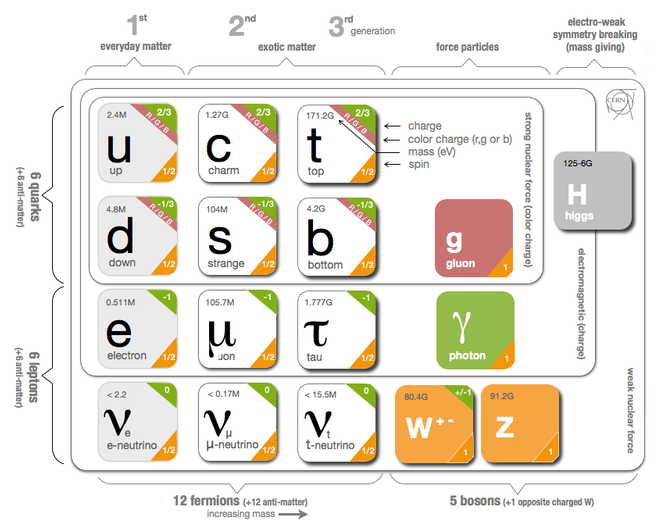
\includegraphics[width=0.95\textwidth]{Figures/HiggsPairProduction/sm.png}
\caption[Standard Model of elementary particles and interactions]{Standard model of elementary particles and interactions~\cite{Purcell:1473657}.}
\label{fig:sm}
\end{figure}

\subsection{The Fermion and Gauge Sectors}
In QFT, the requirement of gauge invariance or symmetry of the Lagrangian density under local phase transformations of a mathematical group introduces the presence of massless boson fields, which are interpreted as the quanta mediating the interaction. One example of a gauge QFT is quantum electrodynamics (QED). The predictions of QED have been successfully tested by very high-precision experiments~\cite{Karshenboim:2005iy}. The Lagrangian density of the electron field ($\Psi$) interacting with an electromagnetic field is defined as $\mathrm{\mathcal{L}_{QED}=-\frac{1}{4}F_{\mu\nu}F^{\mu\nu} + i\overline{\Psi} D_{\mu} \gamma^{\mu} \Psi - m_{e}\overline{\Psi}\Psi }$, where $\mathrm{F_{\mu\nu}=\partial_{\mu}A_{\nu}-\partial_{\nu}A_{\mu} }$ is the electromagnetic field strength, $\mathrm{A_{\mu}}$ is the photon field introduced by gauge invariance, $\mathrm{ D_{\mu}=\partial_{\mu}-iqA_{\mu} }$ is the covariant derivative, and q is the absolute value of electron electric charge. The $\mathrm{\mathcal{L}_{QED}}$ Lagrangian density is invariant under the $\mathrm{U(1)_{Q}}$ group local transformations of the electron and photon fields: $\mathrm{\Psi^{'}(x)=e^{iq\alpha(x)}\Psi(x)}$ and $\mathrm{A^{'}_{\mu} = A_{\mu} - \frac{1}{q}\partial_{\mu}\alpha(x)}$, respectively. Note that $\mathrm{\mathcal{L}_{QED}}$ is not invariant if there is mass term associated to the photon field is imposed (e.g. $\frac{1}{2}m_{A}^{2}~A^{\mu}A_{\mu}$)~\cite{peskin,costa,pdg}.

The SM is a generalization of the fundamental interactions under the $\mathrm{SU(3)_{C} \bigotimes SU(2)_{L}\bigotimes U(1)_{Y} }$ group. The strong interaction is studied by quantum chromodynamics (QCD) based on the $\mathrm{SU(3)_{C}}$ color group. In QCD, colored fermion fields (quarks) represented by SU(3) color triplets $\mathrm{q=\icol{q_{1}\\q_{2}\\q_{3}}}$ interact via 8 massless gauge boson fields (gluons) corresponding to the $\mathrm{SU(3)_{C}}$ generators. Both quarks and gluons have three possible color charges: red (r), blue (b) and green (g). The strength of the interaction is quantified by the strong coupling constant $\mathrm{g_{s}}$ (or $\mathrm{\alpha_{s} = \frac{g_{s}}{4\pi}}$). An important result of the QCD formulation is a phenomenon known as asymptotic freedom. At low-energy scales ($Q^{2}$), the value of the $\alpha_{s}$ strength increases, dictating the confinement of quarks and gluons within color-neutral composite particles named as hadrons (e.g. the proton). At high energies scales, the $\alpha_{s}$ strength decreases ($\mathrm{\alpha_{s}<<1}$), allowing the experimental study of the hadron constituents often named partons. The inner structure of hadrons are made of valence quarks, gluons and quark-antiquark pairs, which are described by the Parton Distribution Function (PDF). There are no free quarks observed in nature because they almost instantaneously ($10^{-24}-10^{-23}$s) become part of hadrons within a collimated shower of particles (hadronic jets) through a process named hadronization (except the top quark which decays at $\sim10^{-25}$ s)~\cite{costa,pdg}. 

The electromagnetic and weak interactions are studied in a unified manner by the electroweak (EW) theory based on the $\mathrm{SU(2)_{L}\bigotimes U(1)_{Y} }$ group~\cite{Weinberg:1967tq,Salam:1968rm,Glashow:1961tr}. Experimental measurements show that only fermions with left-handed chirality interact via charged weak interactions. The right-handed (R) and left-handed (L) chirality components of a fermion field $\Psi$ are obtained using projection operators as  $\mathrm{\Psi_{R/L}}=\frac{1\pm\gamma^{5}}{2} \Psi$. In the EW formalism, the massless gauge bosons are $\mathrm{W_{\mu}^{i}(i=1,2,3)}$ and $\mathrm{B_{\mu}}$. They mediate interactions for fermions with non-zero isospin I and hypercharge Y, respectively. The relation between electric charge (Q), third component of isospin ($\mathrm{I_{3}}$) and hypercharge (Y) is $\mathrm{Q=I_{3} + \frac{Y}{2} }$. The left-handed fermions ($I\neq0$) are represented by the SU(2) doublets $\mathrm{\icol{\nu_{\ell} \\ \\ \ell^{-}}_{L}}$ and $\mathrm{\icol{u \\ \\ d }_{L}}$, respectively. The right-handed fermions ($I=0$) are represented by SU(2) singlets ($\mathrm{\ell^{-}_{R}}$, $\mathrm{u_{R}}$ and $\mathrm{d_{R}}$). 

The experimental short range nature of weak interactions implies the existence of massive vector bosons. Furthermore, observed fermions like the electron are massive particles. However, explicit mass terms associated to the gauge boson and fermion fields are forbidden in the EW Lagrangian density due to $\mathrm{SU(2)_{L}\bigotimes U(1)_{Y} }$ gauge symmetry. Therefore, the formulation needs a gauge invariant mechanism to generate these masses~\cite{costa,pdg}.

\subsection{The Scalar Sector}
The Brout-Englert-Higgs (BEH) mechanism solves elegantly the mass-generation paradigm without violating gauge symmetry~\cite{Higgs:1964ia,Englert:1964et,Guralnik:1964eu}. It adds a complex scalar doublet $\Phi$ with a Lagrangian density $\mathrm{\mathcal{L}_{BEH}=\mathcal{D}_{\mu}^{\dagger}\Phi \mathcal{D}^{\mu}\Phi-V(\Phi)}$ , where $\mathrm{V(\Phi) = - \mu^{2} (\Phi^{\dagger}\Phi ) + \lambda (\Phi^{\dagger}\Phi )^{2}  }$ and $\mu^{2},\lambda>0$~\cite{costa,pdg}.

In the BEH mechanism, $\Phi$ develops a vacuum expectation state ($\mathrm{\langle\Phi\rangle_{0}}$) that satisfies the condition: \hbox{$\mathrm{\langle\Phi^{\dagger}\Phi\rangle_{0} = \frac{\mu^{2}} {2\lambda} = \frac{\nu^{2}}{2}}$}, where $\nu$ is known as the vacuum expectation value (vev). This leads to a `spontaneous' breaking of the electroweak symmetry group $\mathrm{SU(2)_{L}\bigotimes U(1)_{Y}}$ (or EWSB) to the electromagnetic group $\mathrm{U(1)_{Q}}$ with a massless photon, and generating the masses to the charged- and neutral-current weak bosons W$^{\pm}$ and Z, respectively. Furthermore, a real scalar field named the Higgs field H is introduced with its massive particle, popularly known as the Higgs boson. Table~\ref{Tab:higgs} summarizes the BEH Lagrangian terms after EWSB. Finally, charged fermion fields acquire masses through Higgs-fermion Yukawa interactions seen Figure~\ref{fig:hinteractions}~E), where fermion masses are given by $\mathrm{m_{f}=\frac{y_{f}\nu}{\sqrt{2}}}$, and $\mathrm{y_{f}}$ is the associated Yukawa coupling. Neutrino fields remain massless in the theory~\cite{costa,pdg}.

One important prediction is the structure of the Higgs boson potential (See Table~\ref{Tab:higgs}) with the associated cubic and quartic Higgs self-interactions via the self-couplings $\mathrm{\lambda_{HHH}}$ and $\mathrm{\lambda_{HHHH}}$, respectively. These self-interactions are responsible for the Higgs boson mass $\mathrm{m_{H}}$. The Higgs self-couplings are connected to the Higgs boson mass and the vev by the relation $\mathrm{\lambda_{HHH} =\lambda_{HHHH} = \frac{m_{H}^{2}} { 2 {\nu}^{2}}}$. The experimental confirmation of this relation is crucial to our understanding of the BEH mechanism and a test of the internal consistency of the SM formulation. The Higgs boson interactions predicted by the SM are illustrated in Figure~\ref{fig:hinteractions}~\cite{costa,pdg}.

\begin{table}[!htb]
\centering
\caption[BEH Lagrangian terms after the spontaneous eletroweak symmetry breaking (EWSB)]{BEH Lagrangian terms after the spontaneous eletroweak symmetry breaking (EWSB). The following variables are used  where V = W, Z: Higgs boson mass ($\mathrm{m_{H}}$), W$^{\pm}$ boson mass ($\mathrm{m_{W}}$), Z boson mass ($\mathrm{m_{Z}}$), coupling $\mathrm{g_{HVV}=\frac{2m_{V}^{2}}{\nu} }$, coupling $\mathrm{g_{VVHH}=\frac{m_{V}^{2}}{\nu^{2}}}$, and coupling $\mathrm{\lambda=\lambda_{HHH} = \lambda_{HHHH} = \frac{m_{H}^{2}} { 2 {\nu}^{2}}}$.}\label{Tab:higgs}
\begin{tabularx}{\textwidth}{XXXX}
\hline
$\mathrm{\mathcal{L}_{BEH}}$ terms after EWSB & Meaning \\
\hline
$\mathrm{\frac{1}{2}(\partial_{\mu}H)(\partial^{\mu}H)}$ & Higgs kinematic term \\[1pt]
$\mathrm{-\frac{1}{2}m_{H}^{2}H^{2} -\nu\lambda_{HHH} H^{3} -\frac{1}{4}\lambda_{HHHH} H^{4} + \frac{1}{4}\lambda \nu^{4}}  $ & Higgs potential term and self-interactions  \\[1pt]
$\mathrm{+ m_{W}^{2} H W_{\mu}^{-} W^{+,\mu} + g_{HWW} H W_{\mu}^{-} W^{+,\mu} }$ & $W^{\pm}$ mass term and HWW interaction \\[1pt]
$\mathrm{+\frac{1}{2}m_{Z}^{2}Z_{\mu}Z^{\mu} + \frac{1}{2} g_{HZZ}H Z_{\mu}Z^{\mu}}$  & Z mass term and HZZ interaction\\[1pt]
$\mathrm{+g_{WWHH} H^{2} W_{\mu}^{-} W^{+,\mu} }$ & WWHH quartic interaction\\[1pt]
$\mathrm{+\frac{1}{2} g_{ZZHH}H^{2} Z_{\mu}Z^{\mu} }$ & ZZHH quartic interaction\\[1pt]
\hline
\end{tabularx}
\end{table}

\begin{figure}[htp!]
\captionsetup[subfigure]{justification=centering}
\centering
\subfloat[]{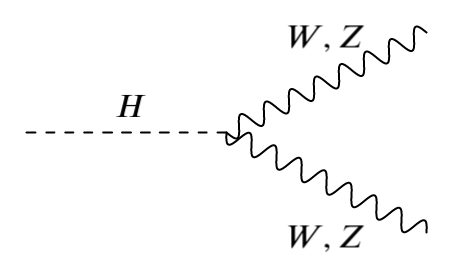
\includegraphics[width=0.30\textwidth]{Figures/HiggsPairProduction/ihvv.png}}
\subfloat[]{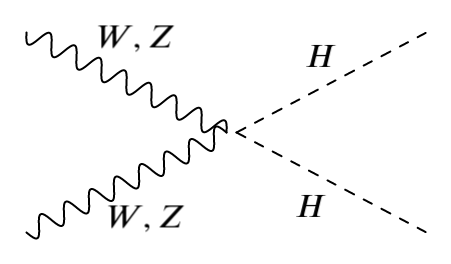
\includegraphics[width=0.30\textwidth]{Figures/HiggsPairProduction/ihhvv.png}}\\
\subfloat[]{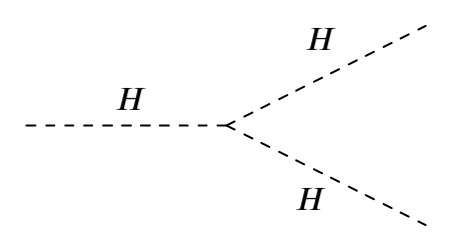
\includegraphics[width=0.30\textwidth]{Figures/HiggsPairProduction/ihhh.png}}
\subfloat[]{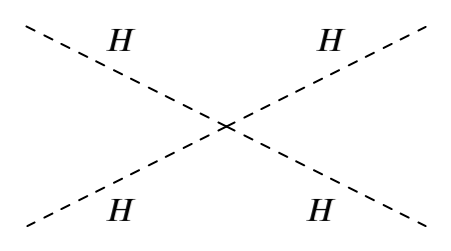
\includegraphics[width=0.30\textwidth]{Figures/HiggsPairProduction/ihhhh.png}}
\subfloat[]{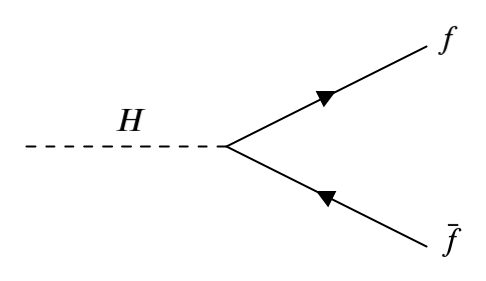
\includegraphics[width=0.30\textwidth]{Figures/HiggsPairProduction/ihf.png}}
\caption[Predicted interactions of the Higgs boson with fermions and vector bosons]{Predicted interactions of the Higgs boson (H) with fermions (f) and vector bosons (V): A) HVV interaction, B) HHVV interaction, C) HHH self-interaction, D) HHHH self-interaction, and E) Higgs-fermion Yukawa interaction.}
\label{fig:hinteractions}
\end{figure}

\subsection{The Higgs Boson}
On July $\mathrm{4^{th}}$ 2012, the CMS and ATLAS Collaborations at the LHC announced the observation of a new resonance with mass around $\hm=125$ GeV and properties compatible with the SM Higgs boson~\cite{atlashiggs,cmshiggs}.  Since then, both collaborations have performed associated precision measurements using 7, 8 and 13 TeV pp collision data, which continue to establish it as the fundamental scalar predicted by the SM. In what follows is presented a brief summary of the Higgs boson production phenomenology, decay channels, and experimental status. 

% Talk about the Higgs boson properties
\subsubsection{Production mechanisms and decay channels}
The value of $\hm$ was the only free parameter left to predict the Higgs boson phenomenology. Given that $\hm$ is known, then the production mechanisms and decays are fully determined. The Higgs boson has several production mechanisms. Gluon fusion (ggF-H) is the main production mode, and then the vector-boson fusion (VBF-H) follows it, with a production cross section of approximately one order of magnitude smaller. Then, the subdominant production modes are the following: associated production with a W or a Z boson (VH) and associated production with a top quark pair ($\mathrm{t\overline{t}H}$), among others. Examples of representative LO diagrams are shown in Figure~\ref{fig:hdiagrams}. In addition, Table~\ref{tab:higgsmodes} presents the theoretical production cross section for several modes. 

\begin{table}[htb]
\centering
\caption[Higgs boson production cross section and relative uncertainties]{\label{tab:higgsmodes} Higgs boson production cross section (in pb) and relative uncertainties (theory, PDF,$\alpha_{S}$) for several Higgs boson ($\mathrm{m_{H}=~125~GeV}$) production modes at $\sqrt{s}=$13 and 14 TeV proton-proton collisions~\cite{pdg}. The order of QCD (EW) calculation is N3LO (NLO) for ggF and NNLO (NLO) for the others.}
\begin{tabularx}{\textwidth}{XXXXXXX}
\hline
$\sqrt{s}$ [TeV] & ggF-H                          &      VBF-H                  & WH                         & ZH                         & $\mathrm{t\overline{t}H}$ & total \\
\hline
13 &  48.6$^{+4.4\%}_{-7.0\%}$ &  3.78$^{+2.2\%}_{-2.2\%}$ &  1.37$^{+2.6\%}_{-2.6\%}$  &  0.88$^{+4.1\%}_{-3.5\%}$  & 0.50$^{+6.8\%}_{-9.9\%}$ & 55.1 \\[0pt]
14 &  54.7$^{+4.4\%}_{-7.0\%}$ &  4.28$^{+2.2\%}_{-2.2\%}$ &  1.51$^{+1.9\%}_{-2.0\%}$  &  0.99$^{+4.1\%}_{-3.7\%}$  & 0.60$^{+6.9\%}_{-9.8\%}$ & 62.1 \\[0pt]
\hline
\end{tabularx}
\end{table}

\begin{figure}[ht!]
\captionsetup[subfigure]{justification=centering}
\centering
\subfloat[]{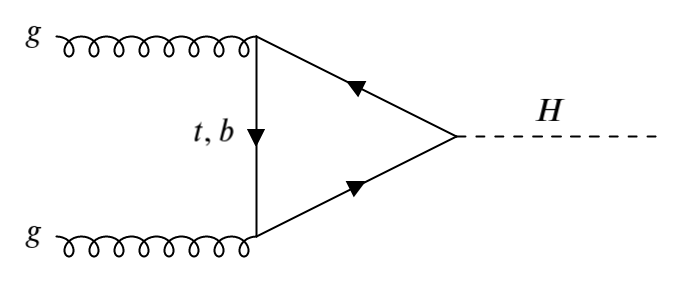
\includegraphics[width=0.33\textwidth]{Figures/HiggsPairProduction/ggfh.png}}
\subfloat[]{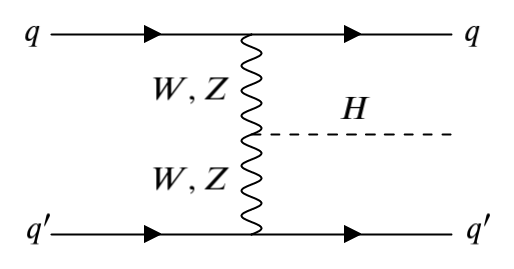
\includegraphics[width=0.25\textwidth]{Figures/HiggsPairProduction/vbfh.png}}\\
\subfloat[]{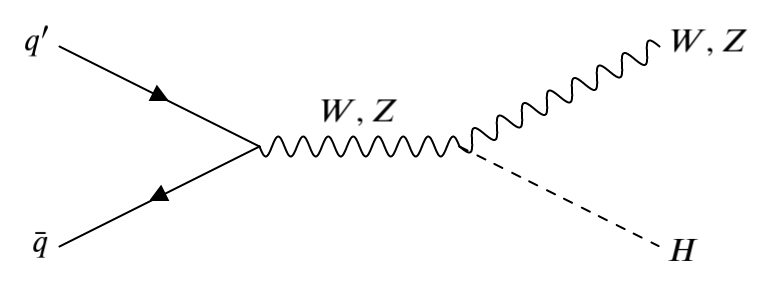
\includegraphics[width=0.33\textwidth]{Figures/HiggsPairProduction/vh.png}}
\subfloat[]{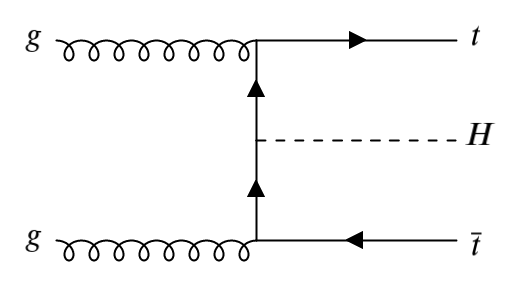
\includegraphics[width=0.25\textwidth]{Figures/HiggsPairProduction/tth.png}}\\
\caption[Examples of leading order diagrams contributing to the Higgs boson production]{Examples of leading order diagrams contributing to the Higgs boson production: A) Gluon fusion, B) Vector boson fusion, (C) Associate production with a W or Z boson, (D) Associate production with a top-quark pair.}
\label{fig:hdiagrams}
\end{figure}

The theoretical Higgs boson decay branching ratios to gauge bosons and to some fermions are presented in Table~\ref{tab:higgsbrs}. The Higgs boson decay to a bottom quark pair ($\mathrm{H\rightarrow~b\overline{b}}$) is the dominant decay channel, with around 58.2\% branching ratio. It is important to note that the Higgs boson can indirectly decay into massless particles via intermediate fermion loops: two photons ($\mathrm{H\rightarrow~\gamma\gamma}$), a Z boson and a photon ($\mathrm{H\rightarrow~Z\gamma}$), and two gluons ($\mathrm{H\rightarrow~gg}$).
\begin{table}[ht!]
\centering
\caption[Higgs boson branching ratios and relative uncertainties for several Higgs boson ($\mathrm{m_{H}=~125~GeV}$) decay modes]{\label{tab:higgsbrs} Higgs boson branching ratios and relative uncertainties for several Higgs boson ($\mathrm{m_{H}=~125~GeV}$) decay modes~\cite{pdg}.}
\begin{tabularx}{\textwidth}{XXXX}
\hline
Decay mode                                    & Branching ratio  & Relative uncertainty      \\
\hline
$\mathrm{H\rightarrow\gamma\gamma}$           & 2.22 x $10^{-3}$ & $\pm$2.1\%            \\[0pt]
$\mathrm{H\rightarrow ZZ}$                    & 2.62 x $10^{-2}$ & $\pm$1.5\%            \\[0pt]
$\mathrm{H\rightarrow W^{+}W^{-}}$            & 2.14 x $10^{-1}$ & $\pm$1.5\%            \\[0pt]
$\mathrm{H\rightarrow \tau^{+}\tau^{-}}$      & 6.27 x $10^{-2}$ & $\pm$1.6\%            \\[0pt]
$\mathrm{H\rightarrow b\overline{b}}$         & 5.82 x $10^{-1}$ & $^{+1.2\%}_{-1.3\%}$  \\[0pt]
$\mathrm{H\rightarrow c\overline{c}}$         & 2.89 x $10^{-2}$ & $^{+5.5\%}_{-2.0\%}$  \\[0pt]
$\mathrm{H\rightarrow Z\gamma}$               & 1.53 x $10^{-3}$ & $\pm$5.8\%            \\[0pt]
$\mathrm{H\rightarrow \mu^{+}\mu^{-}}$        & 2.18 x $10^{-4}$ & $\pm$1.7\%            \\[0pt]
\hline
\end{tabularx}
\end{table}

\subsubsection{Experimental Status}
The LHC exploration of the Higgs boson is carried out analyzing a broad range of production mechanisms and decay channels. The most sensitive decay channels for studying the Higgs boson are as follows. The $\mathrm{H\rightarrow~ZZ\rightarrow 4\ell~(\ell=e,\mu)}$ and $\mathrm{H\rightarrow~\gamma\gamma}$ channels have low expected rates but benefit from small background processes and have the best mass resolution ($\sim$1-2\%) due to well-reconstructed final state products. The $\mathrm{H\rightarrow~W^{+}W^{-}\rightarrow\ell^{+}\nu_{\ell}{\ell}^{\prime-}\overline{\nu}_{\ell\prime}}$ channel has relatively better rates, but the unmeasured energy from neutrinos has an impact on the resolution of the mass-related observables, e.g. the transverse mass resolution is $\sim20\%$. The $\mathrm{b\overline{b}}$ ($\tau^{+}\tau^{-}$) decay channel benefits from high rates and intermediate mass resolutions 10\% (15\%), but is affected by large and irreducible background contamination~\cite{pdg}. Challenging channels due to low very rates or large background levels are $\mathrm{H\rightarrow\mu^{+}\mu^{-}}$ and $\mathrm{H\rightarrow c\overline{c}}$, respectively.

In the LHC Run-1 (2009-2012), the ATLAS and CMS collaborations analyzed the pp collision datasets at $\sqrt{s}=7$ and 8~TeV to discover the Higgs boson~\cite{atlashiggs,cmshiggs}. The decay channels involving gauge bosons, $\mathrm{H\rightarrow~ZZ\rightarrow 4\ell~(\ell=e,\mu)}$ and $\mathrm{H\rightarrow\gamma\gamma}$ , contributed with the most significant excesses.  The $\mathrm{H\rightarrow~W^{+}W^{-}\rightarrow~\ell^{+}\nu_{\ell}{\ell}^{\prime-}\overline{\nu}_{\ell\prime}}$, $\mathrm{H\rightarrow\mathrm{b\overline{b}}}$ and $\mathrm{H\rightarrow\tau^{+}\tau^{-}}$ channels were also included but contributed with lower significance~\cite{atlashiggs,cmshiggs}. After that, studies of the spin-parity ($\mathrm{J^{P}}$) quantum numbers revealed the scalar and even-parity nature ($\mathrm{J^{P}=O^{+}}$) of the discovered particle as predicted by the SM~\cite{atlasrun1_hspinparity,cmsrun1_hmassparityspin}. The Run-1 Combined ATLAS and CMS Higgs boson mass measurement yields a value of $\mathrm{m_{H}=125.09\pm~0.24~GeV}$ using $\mathrm{H\rightarrow~ZZ\rightarrow 4\ell~(\ell=e,\mu)}$ and $\mathrm{H\rightarrow\gamma\gamma}$, benefiting from their excellent mass resolution~\cite{atlascmsrun1hmass}.

In the LHC Run-2 (2015-2018), ATLAS and CMS experiments had an excellent operation performance collecting high-quality data at $\sqrt{s}=13$~TeV, corresponding to approximately 6 times the LHC Run-1 dataset integrated luminosity. Measurements of the mass, couplings, differential and fiducial cross sections have been performed with the partial and full dataset by ATLAS~\cite{atlasrun2mes,atlasrun2hmass} and CMS~\cite{cmsrun2mes,cmsbesthmassrun2}. The Higgs boson mass measurement has been performed using the $\mathrm{H\rightarrow~ZZ\rightarrow 4\ell~(\ell=e,\mu)}$ and $\mathrm{H\rightarrow\gamma\gamma}$ decay channels. The distribution of the di-photon invariant mass in the 2016 data is presented in Figure~\ref{fig:LHCHiggsmeasurements}~A). The best mass measurement yields a value of $\mathrm{m_{H}=125.38\pm0.14~GeV}$ from the CMS combination of Run-1 and 2016 datasets~\cite{cmsbesthmassrun2}. 

Both experiments have presented the observation of the Higgs coupling to third generation fermions studying the $\mathrm{H\rightarrow~b\overline{b}}$~\cite{atlasrun2_hbb,cmsrun2_hbb} and $\mathrm{H\rightarrow\tau^{+}\tau^{-}}$~\cite{atlasrun2_htautau,cmsrun2_htautau} decays, and the $\mathrm{ttH}$ production mode~\cite{atlasrun2_tth,cmsrun2_tth}. In particular, the measurement of $\mathrm{H\rightarrow~b\overline{b}}$ decays was believed to be impossible to achieve due to the large multi-jet background and intermediate mass resolution. However, novel analysis methods based on machine learning (ML) were developed for object identification, reconstruction and signal identification, to maximize the search sensitivity. Figure~\ref{fig:LHCHiggsmeasurements} B) illustrates the distribution signal-to-background ratio bins in the $\mathrm{H\rightarrow~b\overline{b}}$ measurement. The CMS experiment found the first evidence for the Higgs coupling to the second generation fermions in the analysis of the $\mathrm{H\rightarrow\mu^{+}\mu^{-}}$ decay channel~\cite{cmsrun2_hmumu}. ATLAS show the first evidence for the $\mathrm{H\rightarrow~(\gamma/Z)^{*}\gamma~\rightarrow\ell\ell\gamma}$ decay channel~\cite{atlasrun2_h_zgamma}. Lastly, both experiments are currently developing methods to measure the $\mathrm{H\rightarrow c\overline{c}}$ decay but the development of more sophisticated methods and more data are needed to measure it in the future~\cite{atlasrun2_hcc,cmsrun2_hcc}. The Figure~\ref{fig:LHCHiggsmeasurements} C) shows the Higgs coupling measurements using CMS Run-2 data.
%Most of the signal significance comes from the analysis of the VH production mode with vector bosons decaying into 0, 1, 2 charged leptons ($\mu$ or e).
\begin{figure}[ht!]
\captionsetup[subfigure]{justification=centering}
\centering
\subfloat[]{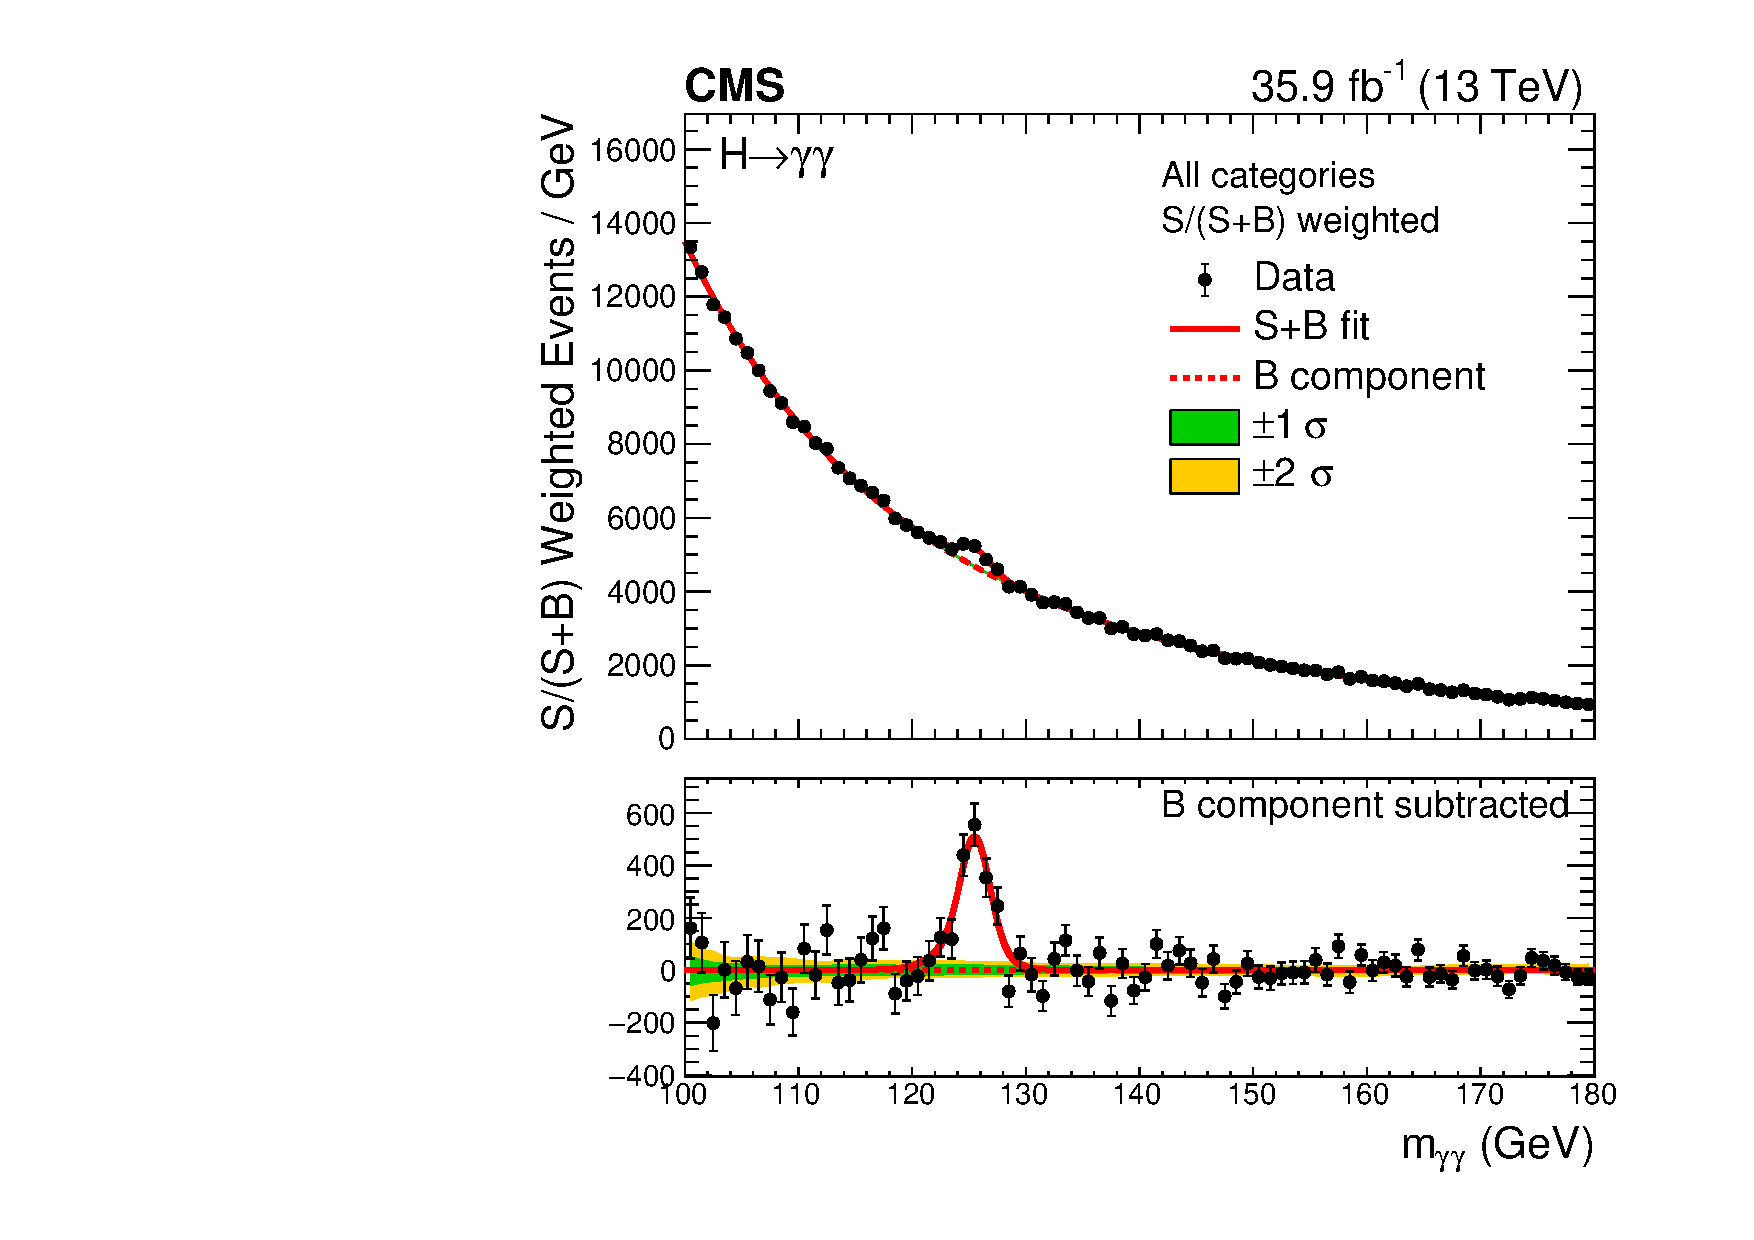
\includegraphics[width=0.32\textwidth]{Figures/HiggsPairProduction/2016higgsggmass.pdf}}
\subfloat[]{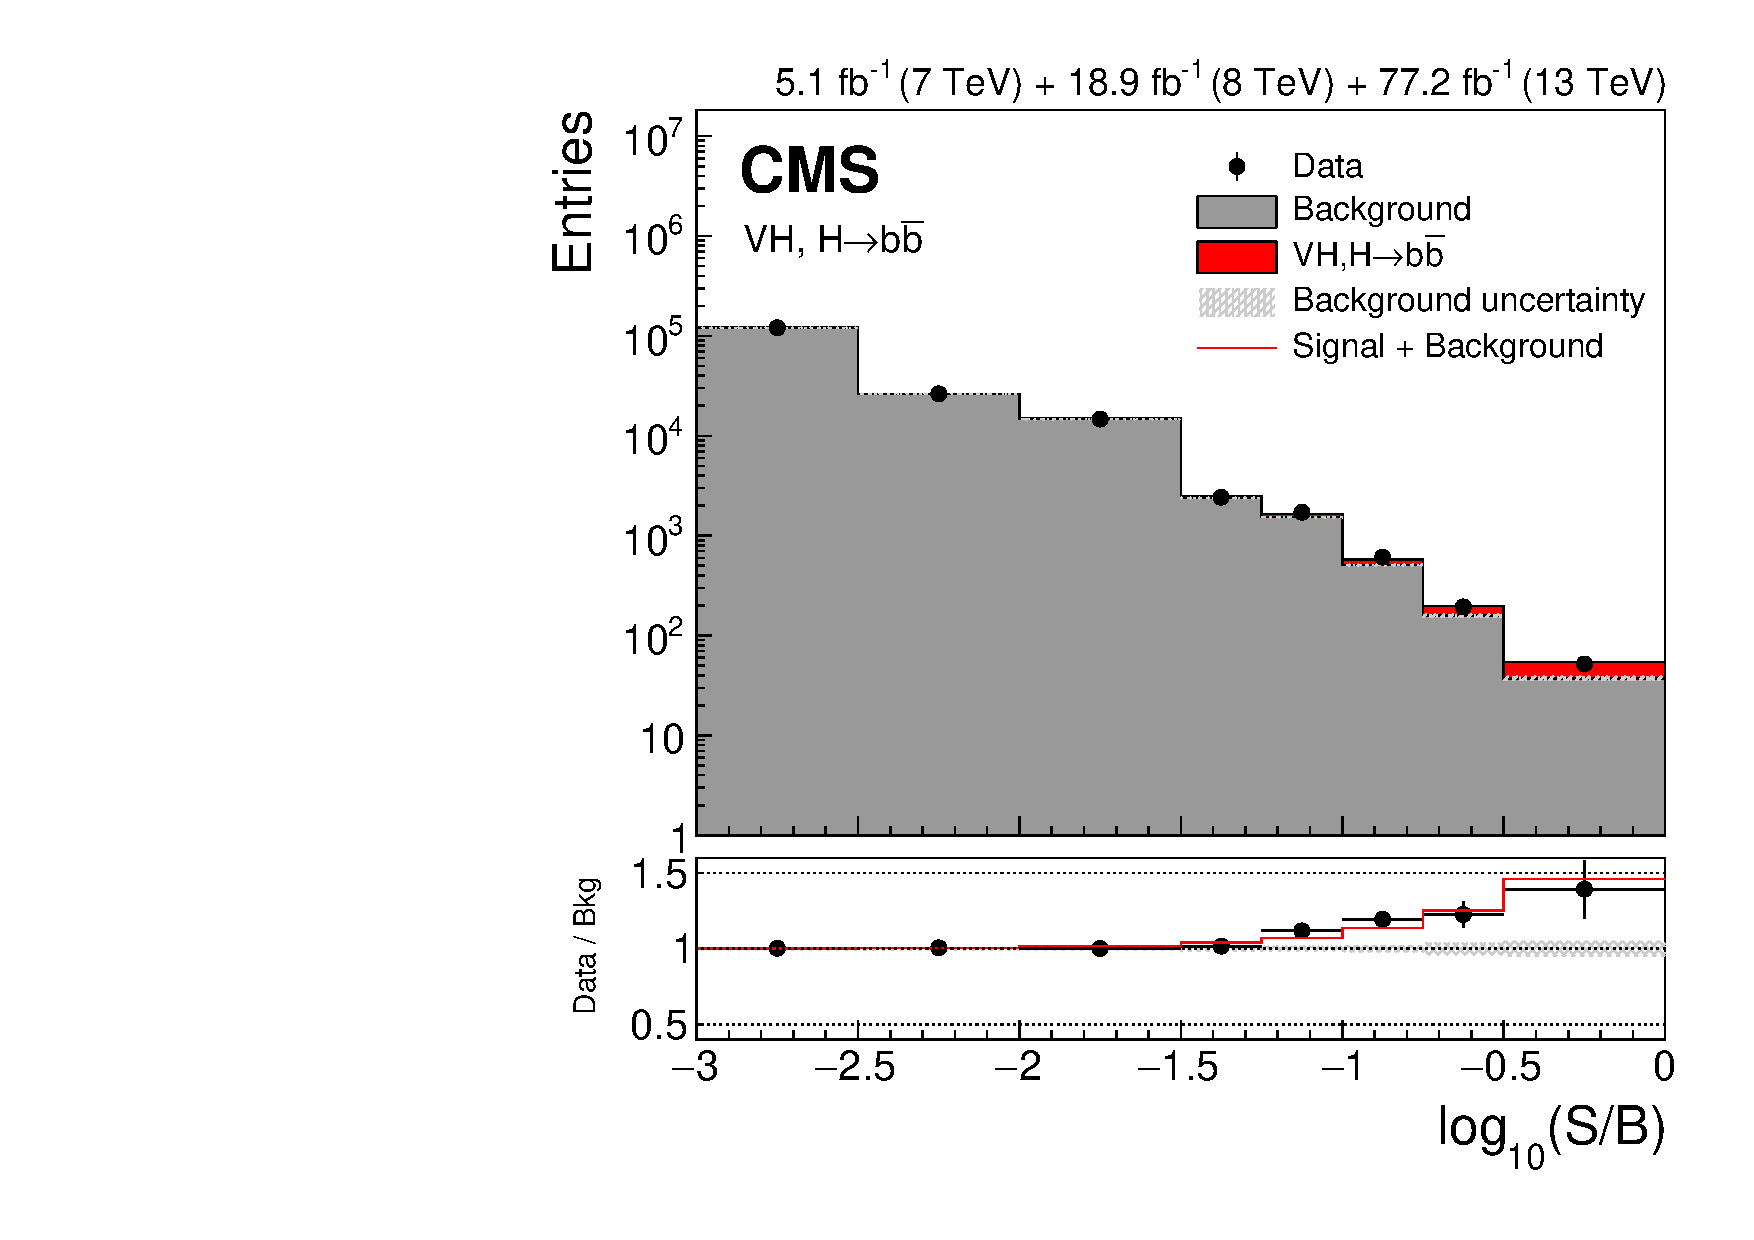
\includegraphics[width=0.32\textwidth]{Figures/HiggsPairProduction/higgsbbsb.pdf}}\\
\subfloat[]{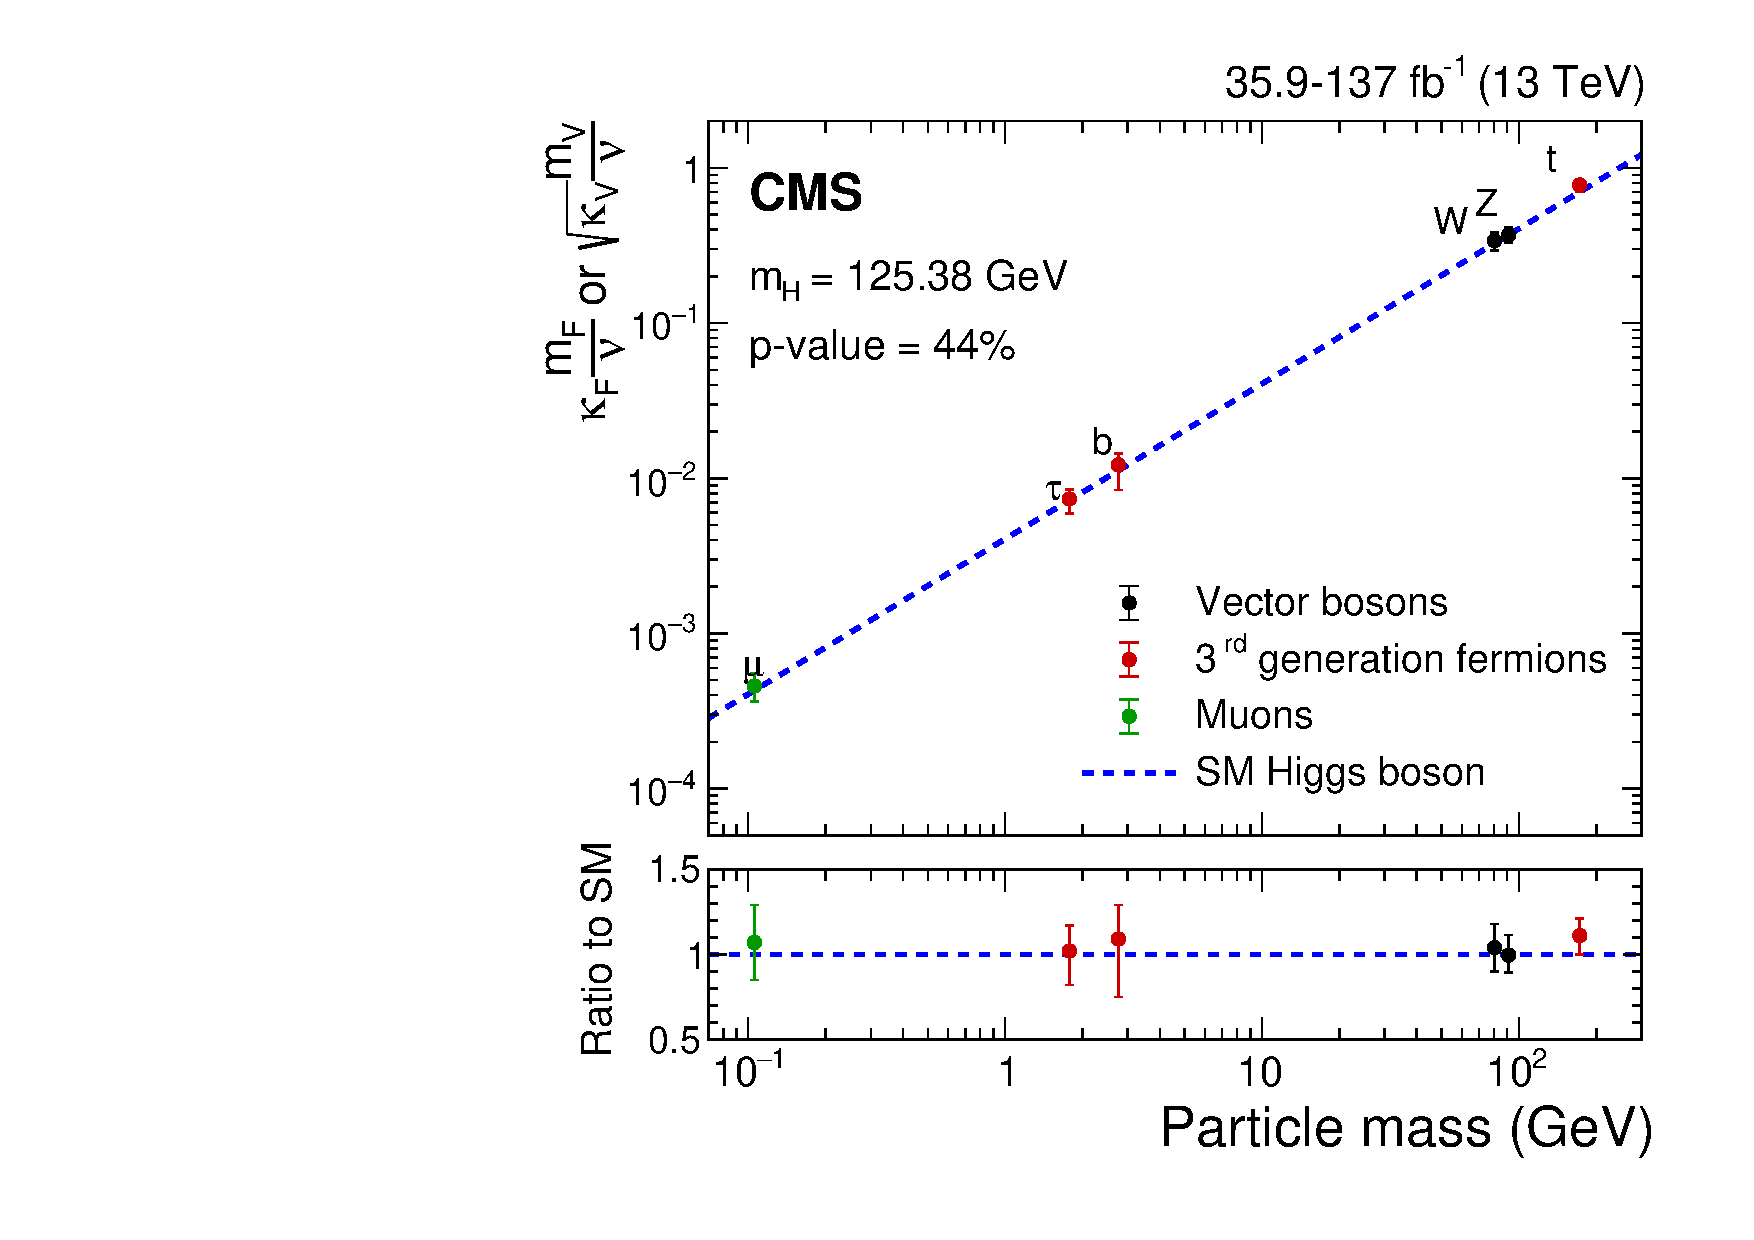
\includegraphics[width=0.32\textwidth]{Figures/HiggsPairProduction/higgscouplingsrun2.pdf}}
\caption[Selected CMS Higgs physics results in Run-2]{Selected CMS Higgs physics results in Run-2. A) Di-photon mass distribution from the 2016 dataset mass measurement~\cite{cmsbesthmassrun2}, B) Distribution of event yields sorted into bins of similar signal-to-background ratio in the observation of Higgs coupling to two bottom-quarks~\cite{cmsrun2_hbb}, C) Measurement of the Higgs couplings~\cite{cmsrun2_hmumu}.}
\label{fig:LHCHiggsmeasurements}
\end{figure}
   
\clearpage
\section{Higgs Boson Pair Production}
This section is a review of the theoretical aspects and phenomenology associated to the Higgs boson pair (HH) production. First, the physics of SM HH production is discussed. Then, the motivation and characteristics of the BSM HH production are summarized. 

\subsection{Standard Model Production}
From the precise measurement of the Higgs boson mass, the value of the Higgs self-couplings are fully predicted. The Higgs trilinear coupling or self-coupling $\mathrm{\lambda_{HHH} = \frac{m_{H}^{2}} { 2 {\nu}^{2}}\sim0.13}$, where, $\nu$ is around 246 GeV from measurements of the Fermi constant $G_{F}$. Non-resonant HH production is the only SM process with direct access to measure $\mathrm{\lambda_{HHH}}$ at the LHC. The main production mechanisms are the following, ordered by their cross section (see Table~\ref{tab:hhxs}): Gluon fusion production (ggF), vector boson fusion production (VBF), associated production with a Z or W boson (VHH) and top quark pairs associated production ($\mathrm{t\overline{t}HH}$). Some representative LO Feynman diagrams for each mode are illustrated in Figure~\ref{fig:hhdiagrams}. Note that single Higgs production has indirect access to the $\mathrm{\lambda_{HHH}}$ coupling via NLO EW corrections~\cite{Degrassi:2016wml,Maltoni:2017ims}.

\begin{table}[htb]
\centering
\caption[Higgs boson pair production cross section (in pb) and relative uncertainties]{\label{tab:hhxs} Higgs boson pair production cross section (in fb) and relative uncertainties for several Higgs boson ($\mathrm{m_{H}=~125~GeV}$) production modes at $\sqrt{s}=$13 and 14 TeV proton-proton collisions~\cite{DiMicco:2019ngk}.}
\begin{tabularx}{\textwidth}{XXX}
\hline
$\sqrt{s}$                  & 13 TeV                               & 14 TeV                                 \\
\hline
$\mathrm{ggF}$              & 31.05$^{+6.0\%}_{-23.0\%}\pm3.0\%$   &  36.69$^{+6.0\%}_{-23.0\%}\pm3.0\%$     \\[0pt]
$\mathrm{VBF}$              &   1.73$^{+0.03\%}_{-0.04\%}\pm2.1\%$ &  2.05$^{+0.03\%}_{-0.04\%}\pm2.1\%$    \\[0pt]
$\mathrm{ZHH}$              &  0.363$^{+3.4\%}_{-2.7\%}\pm1.9\%$   &  0.415$^{+3.5\%}_{-2.7\%}\pm1.8\%$     \\[0pt]
$\mathrm{W^{+}HH}$          &  0.329$^{+0.32\%}_{-0.41\%}\pm2.2\%$ &  0.369$^{+0.33\%}_{-0.39\%}\pm2.1\%$   \\[0pt]
$\mathrm{W^{-}HH}$          &  0.173$^{+1.2\%}_{-1.3\%}\pm2.8\%$   &  0.198$^{+1.2\%}_{-1.3\%}\pm2.7\%$     \\[0pt]
$\mathrm{t\overline{t}HH}$  &  0.773$^{+1.5\%}_{-4.3\%}\pm3.2\%$   &  0.949$^{+1.7\%}_{-4.5\%}\pm3.1\%$     \\[0pt]
\hline
\end{tabularx}
\end{table}

In the dominant mode, gluon fusion, Higgs boson pairs proceed from quantum loops involving mainly top-quarks (and a small b-quark contribution). At LO, a triangle-loop diagram and a box-loop diagram contribute to the ggF mode physics (see Figure~\ref{fig:hhdiagrams}~A)). The triangle-loop diagram contains the Higgs self-coupling $\mathrm{\lambda_{HHH}}$, while the box diagram contains the top quark Yukawa coupling ($\mathrm{y_{t}}$). There is a large negative interference between the two loop diagrams, resulting in a very small production cross section. The individual contributions to the cross section from the box, triangle and their interference are illustrated as function HH invariant mass in Figure~\ref{fig:hhmcont}. The triangle or self-interaction diagram contribution is mostly located at low HH mass values (i.e. soft spectrum) and is largely suppressed by the interference contribution.

\begin{figure}[htp!]
\centering
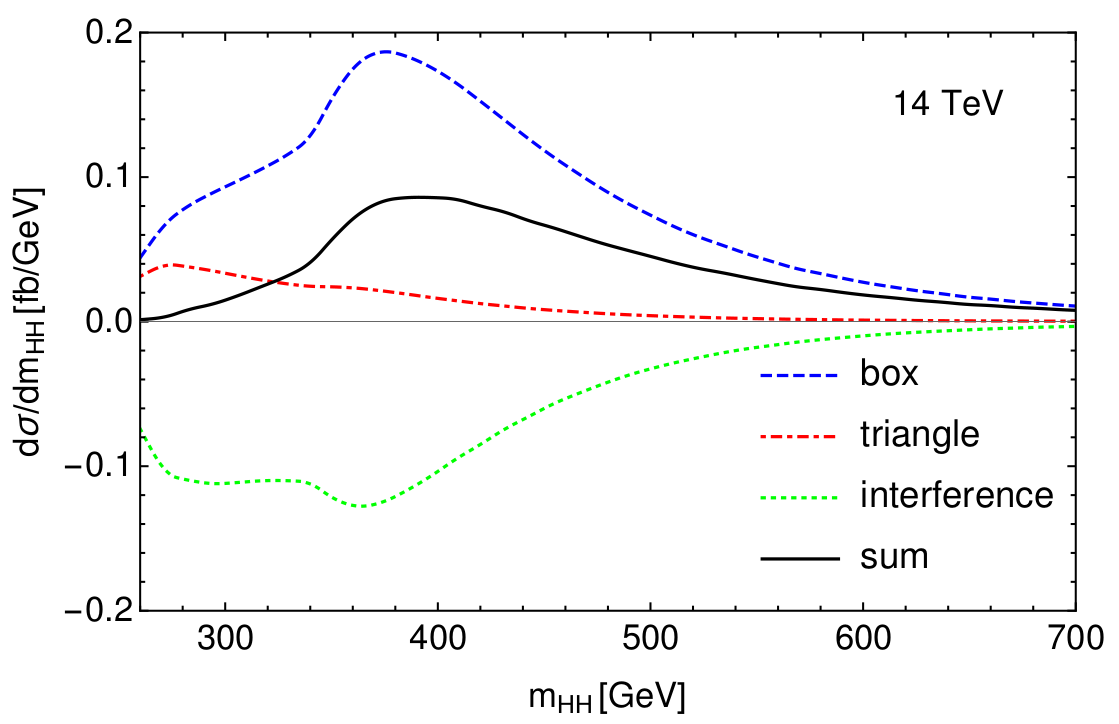
\includegraphics[width=1.0\textwidth]{Figures/HiggsPairProduction/mhhcont.png}
\caption[Differential cross section distribution as a function of the Higgs boson invariant mass]{Differential cross section distribution as a function of the Higgs boson invariant mass at leading order~\cite{DiMicco:2019ngk}. The contributions to the gluon fusion production cross section (black line) are presented: box (dashed blue), triangle (dashed red), interference (dashed green).}
\label{fig:hhmcont}
\end{figure}

The secondary production mode, vector boson fusion (VBF), has three LO contributing diagrams shown in Figure~\ref{fig:hhdiagrams}~B). The VBF production cross section is approximately one order of magnitude smaller than the ggF one but has a very characteristic signature with two quark hadronic jets with large invariant mass and separation in the final state. Besides having an extra handle on the $\mathrm{\lambda_{HHH}}$ coupling, this process has a unique access to study the interaction between two vector bosons and two Higgs bosons through the $\mathrm{g_{HHVV}}$ coupling. Moreover, this mode has access to the interaction between the Higgs boson and two vector bosons via the $\mathrm{g_{HVV}}$ coupling. 

\begin{figure}[ht]
\captionsetup[subfigure]{justification=centering}
    \centering
      \begin{subfigure}{\textwidth}
  \centering
          \caption{}
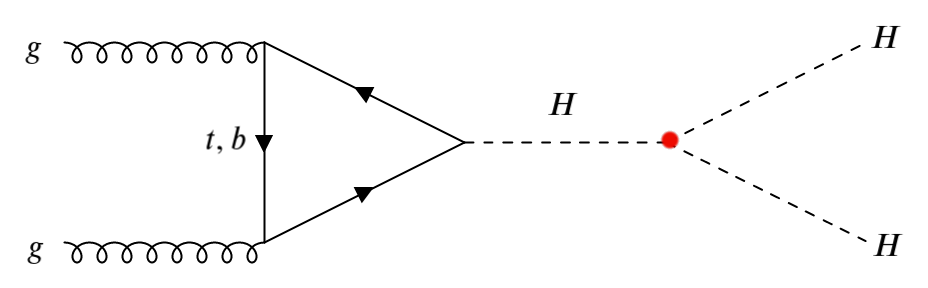
\includegraphics[width=0.40\textwidth]{Figures/HiggsPairProduction/ggf1.png}
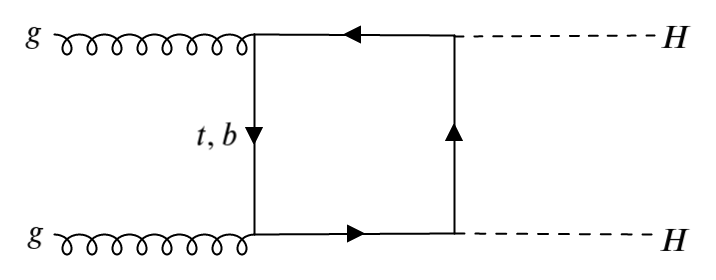
\includegraphics[width=0.30\textwidth]{Figures/HiggsPairProduction/ggf2.png}\\
      \end{subfigure}
      \begin{subfigure}{\textwidth}
  \centering
          \caption{}
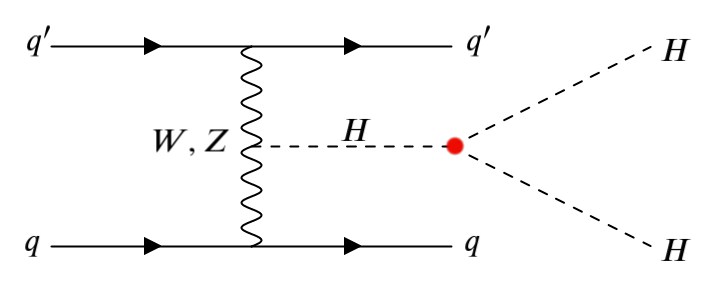
\includegraphics[width=0.32\textwidth]{Figures/HiggsPairProduction/vbf2.png}
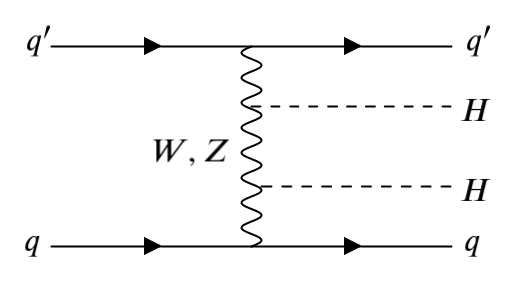
\includegraphics[width=0.23\textwidth]{Figures/HiggsPairProduction/vbf1.png}
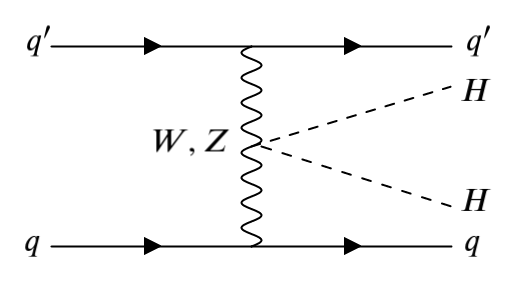
\includegraphics[width=0.23\textwidth]{Figures/HiggsPairProduction/vbf3.png}\\
      \end{subfigure}
      \begin{subfigure}{\textwidth}
  \centering
          \caption{}
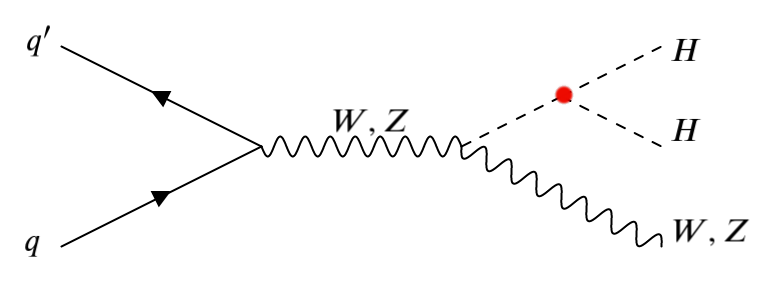
\includegraphics[width=0.32\textwidth]{Figures/HiggsPairProduction/vhh1.png}
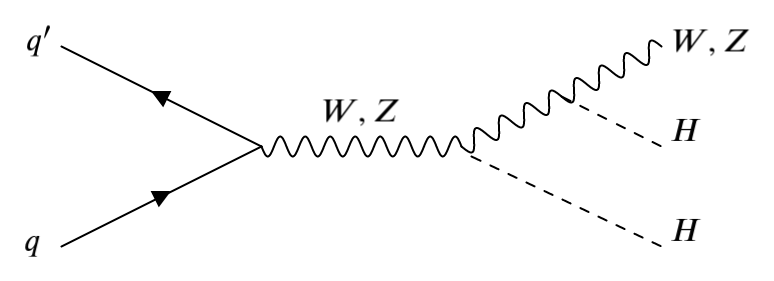
\includegraphics[width=0.32\textwidth]{Figures/HiggsPairProduction/vhh2.png}
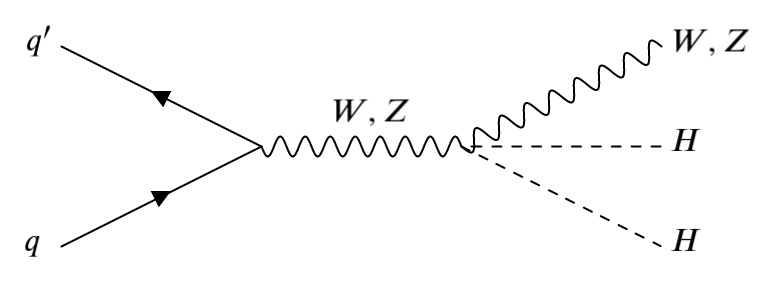
\includegraphics[width=0.32\textwidth]{Figures/HiggsPairProduction/vhh3.png}\\
      \end{subfigure}
      \begin{subfigure}{\textwidth}
  \centering
          \caption{}
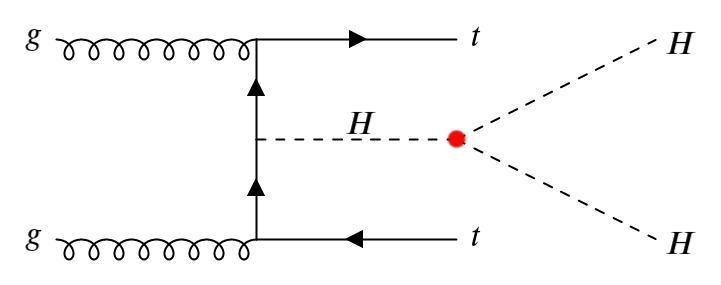
\includegraphics[width=0.30\textwidth]{Figures/HiggsPairProduction/tthh1.png}
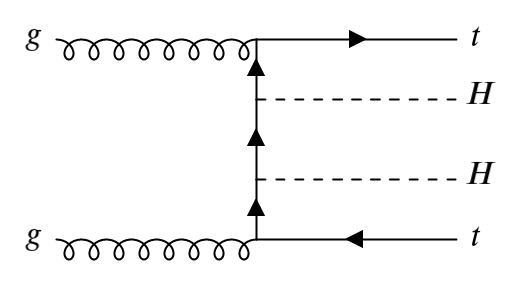
\includegraphics[width=0.22\textwidth]{Figures/HiggsPairProduction/tthh2.png}\\
      \end{subfigure}
\caption[Examples of leading order (LO) diagrams contributing to the Higgs boson pair production mode mechanisms]{Examples of leading order (LO) diagrams contributing to the Higgs boson pair production mode mechanisms. A) Gluon fusion, B) Vector boson fusion C) Associate production with a W or Z boson, D) Associate production with top-quark pair. The red circle represents the Higgs self-coupling $\mathrm{\lambda_{HHH}}$.}
\label{fig:hhdiagrams}
\end{figure}

\subsection{Beyond the Standard Model Production} \label{hh:BSMcouplings}
Although the SM have been successfully in predicting the measurements at particle colliders, it does not provide explanations to many experimental and theoretical aspects about nature. Many of them are connected to the scalar sector, which hints that BSM physics is hidden there. From the theoretical point of view, there is no fundamental symmetry to protect the Higgs boson mass from quadratically divergent radiative corrections~\cite{pdg}. Furthermore, a metastable scalar potential appears to be favored based on the measured Higgs boson and top-quark masses, challenging the long-term stability of the Universe~\cite{Elias-Miro:2011sqh}.

Many BSM physics scenarios are able to regulate the shortcomings of the SM. Some of these models have extra singlets~\cite{Robens,Dawson:2015haa}, extra doublets inspired by the next-to-minimal supersymmetric extension of the SM(NMSSM)~\cite{Ellwanger:2009dp,Djouadi}, or warped extra-dimensions with a new scalar or a graviton~\cite{RandallSundrum,Oliveira:2014kla}.  A broad class of these models predict the production of new particles (X) that can subsequently decay in a sizeable branching fraction to a pair of Higgs boson ($\mathrm{X\rightarrow~HH}$)~as illustrated in the diagrams in Figure~\ref{fig:resonances}. At the LHC, one can probe these BSM models using a common experimental signature consisting of an enhancement of the cross section at the X mass ($\mathrm{m_{X}}$). The studied masses range from 250 GeV ($\mathrm{m_{X}>2~m_{H}}$) to a few TeVs. Recent theoretical work has also highlighted the possibility of spectacular multi-scalar resonant decays into a new scalar (Y) and a Higgs boson ($\mathrm{X\rightarrow YH}$), and a Higgs boson triplet ($\mathrm{X\rightarrow YH\rightarrow HHH}$) ~\cite{Ellwanger:2017skc,Robens:2019kga}.

\begin{figure}[htp!]
\centering
\captionsetup[subfigure]{justification=centering}
\subfloat[]{\centering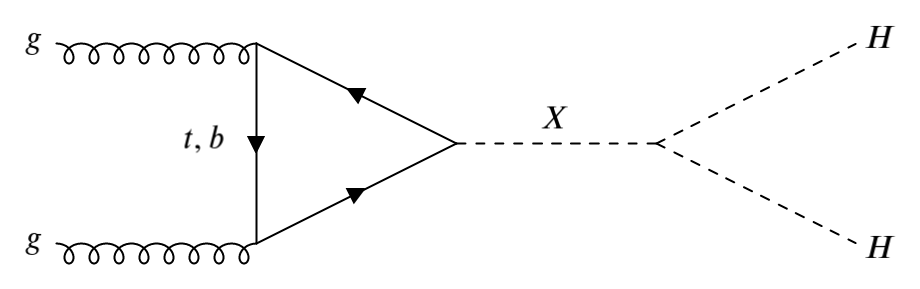
\includegraphics[width=0.50\textwidth]{Figures/HiggsPairProduction/xggf.png}}
\subfloat[]{\centering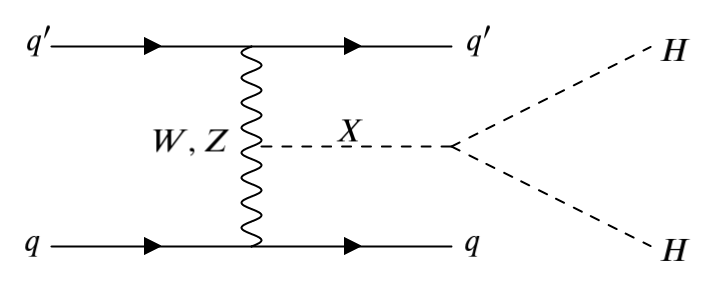
\includegraphics[width=0.43\textwidth]{Figures/HiggsPairProduction/xvbf.png}}\\
\caption[Diagrams of production of a new resonances decaying to a Higgs boson pair at the LHC]{Diagrams of production of a new resonances decaying to a Higgs boson pair at the LHC: A) Gluon fusion production mode, and B) Vector boson production mode.}
\label{fig:resonances}
\end{figure}

If the scale of the new physics is beyond the direct reach of the LHC, the effects of the new particles and their interactions within quantum loops may result in modifications of the HH production cross section and kinematics. These modifications can be parametrized with respect to the SM value through coupling modifiers($\kappa$). For instance, anomalous Higgs self-coupling, $\mathrm{g_{HVV}}$ coupling and  $\mathrm{g_{VVHH}}$ coupling have the modifiers $\mathrm{\kappa_{\lambda}=\lambda_{HHH}/\lambda^{SM}_{HHH}}$, $\mathrm{\kappa_{V}}$, and $\mathrm{\kappa_{2V}}$ , respectively. Figure~\ref{fig:klambdaxs} presents the dependence of the cross section for different production modes as a function of the $\mathrm{\kappa_{\lambda}}$ modifier (assuming other couplings are set to their SM values). The ggF mode cross section has a quadratic $\mathrm{\kappa_{\lambda}}$-dependence, with a minimum at around 2.45 (maximal interference effect). 

\begin{figure}[ht]
\centering
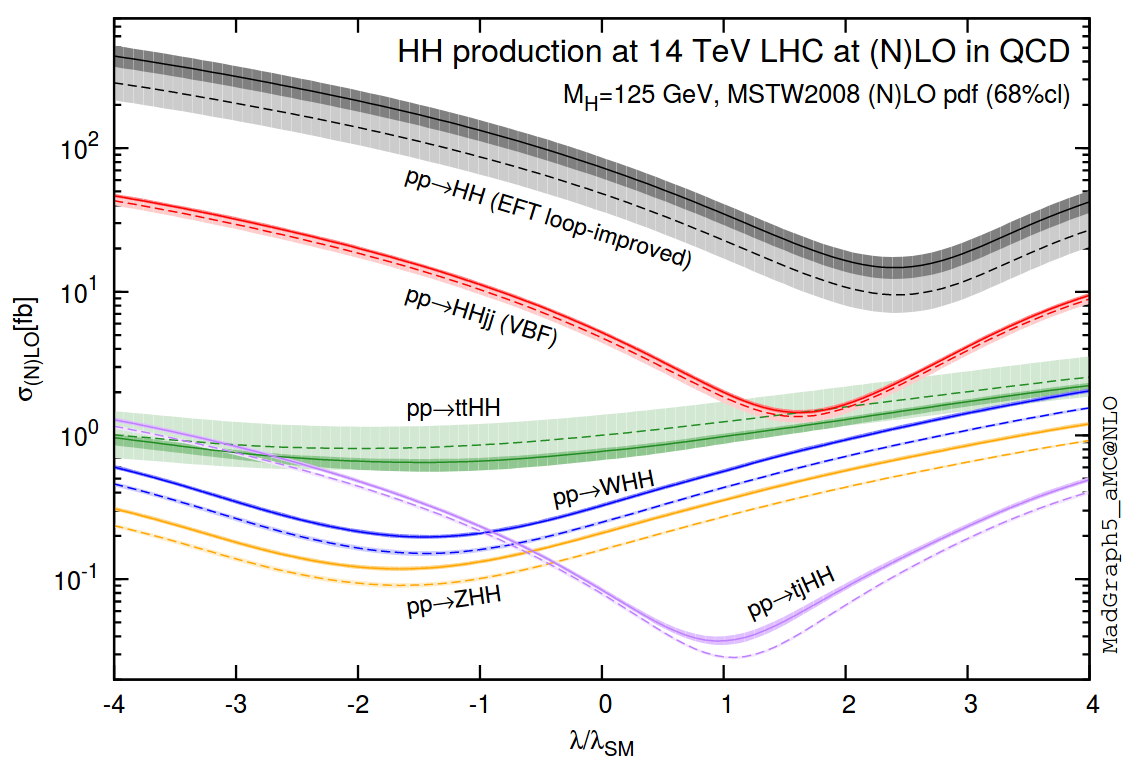
\includegraphics[width=0.9\textwidth]{Figures/HiggsPairProduction/klambdaxs.png}
\caption[Higgs boson pair production cross section at $\sqrt{s}=14$ TeV LHC proton-proton collisions for various modes]{Higgs boson pair production cross section at $\sqrt{s}=14$ TeV LHC proton-proton collisions for various modes calculated at the LO and NLO precision in QCD, as a function of the Higgs self-coupling with respect to the SM ($\mathrm{\lambda/\lambda_{SM}}$)~\cite{Frederix:2014hta}. The dashed (solid) lines and light- (dark-)color bands correspond to the LO (NLO) results and to the scale and PDF uncertainties added linearly.}
\label{fig:klambdaxs}
\end{figure}

BSM $\mathrm{\kappa_{\lambda}}$ values ($\mathrm{\kappa_{\lambda}\neq1}$)  modify the kinematic properties of the Higgs boson pair. This effect is illustrated on Figure~\ref{fig:mhhvariation} A), where the HH invariant mass spectrum for different values of the $\mathrm{\kappa_{\lambda}}$ modifier in the ggf mode is shown. The softest spectrum (experimentally challenging due to event selection thresholds), corresponds to $\mathrm{\kappa_{\lambda}=5}$. Note that the case where mostly the triangle diagram contributes to the HH production cross section ($\mathrm{\kappa_{\lambda}=20}$) has a soft spectrum, whereas the case of box diagram ($\mathrm{\kappa_{\lambda}=20}$) has an intermediate mass spectrum. For the $\mathrm{\kappa_{\lambda}=2.45}$ case, a spectrum with a low mass peak and intermediate mass peak is seen.

In the VBF mode, the amplitude of the longitudinal scattering of vector bosons contributing to the production cross section depends on the center-of-mass energy ($\mathrm{\hat{s}}$) and $\mathrm{\kappa_{V}}$, and $\mathrm{\kappa_{2V}}$ as $\mathcal{A}(\mathrm{V_{L}V_{L}\rightarrow~HH)}\simeq \frac{\mathrm{\hat{s}}}{v^{2}}(\kappa_{2V}-\kappa_{V}^{2})$. Note that this amplitude is suppressed in the SM ($\mathrm{\kappa_{2V}=\kappa_{V}=1}$), but is present for cases when $\mathrm{\kappa_{2V}\neq\kappa_{V}^{2}}$. Consequently, the effect of BSM physics may manifest as an enhancement at high HH masses, illustrated in Figure~\ref{fig:mhhvariation} B) for anomalous $\mathrm{\kappa_{2V}}$ values 0 (no VVHH interaction) and 2 (enhanced VVHH interaction).

\begin{figure}[htp!]
\centering
\captionsetup[subfigure]{justification=centering}
\subfloat[]{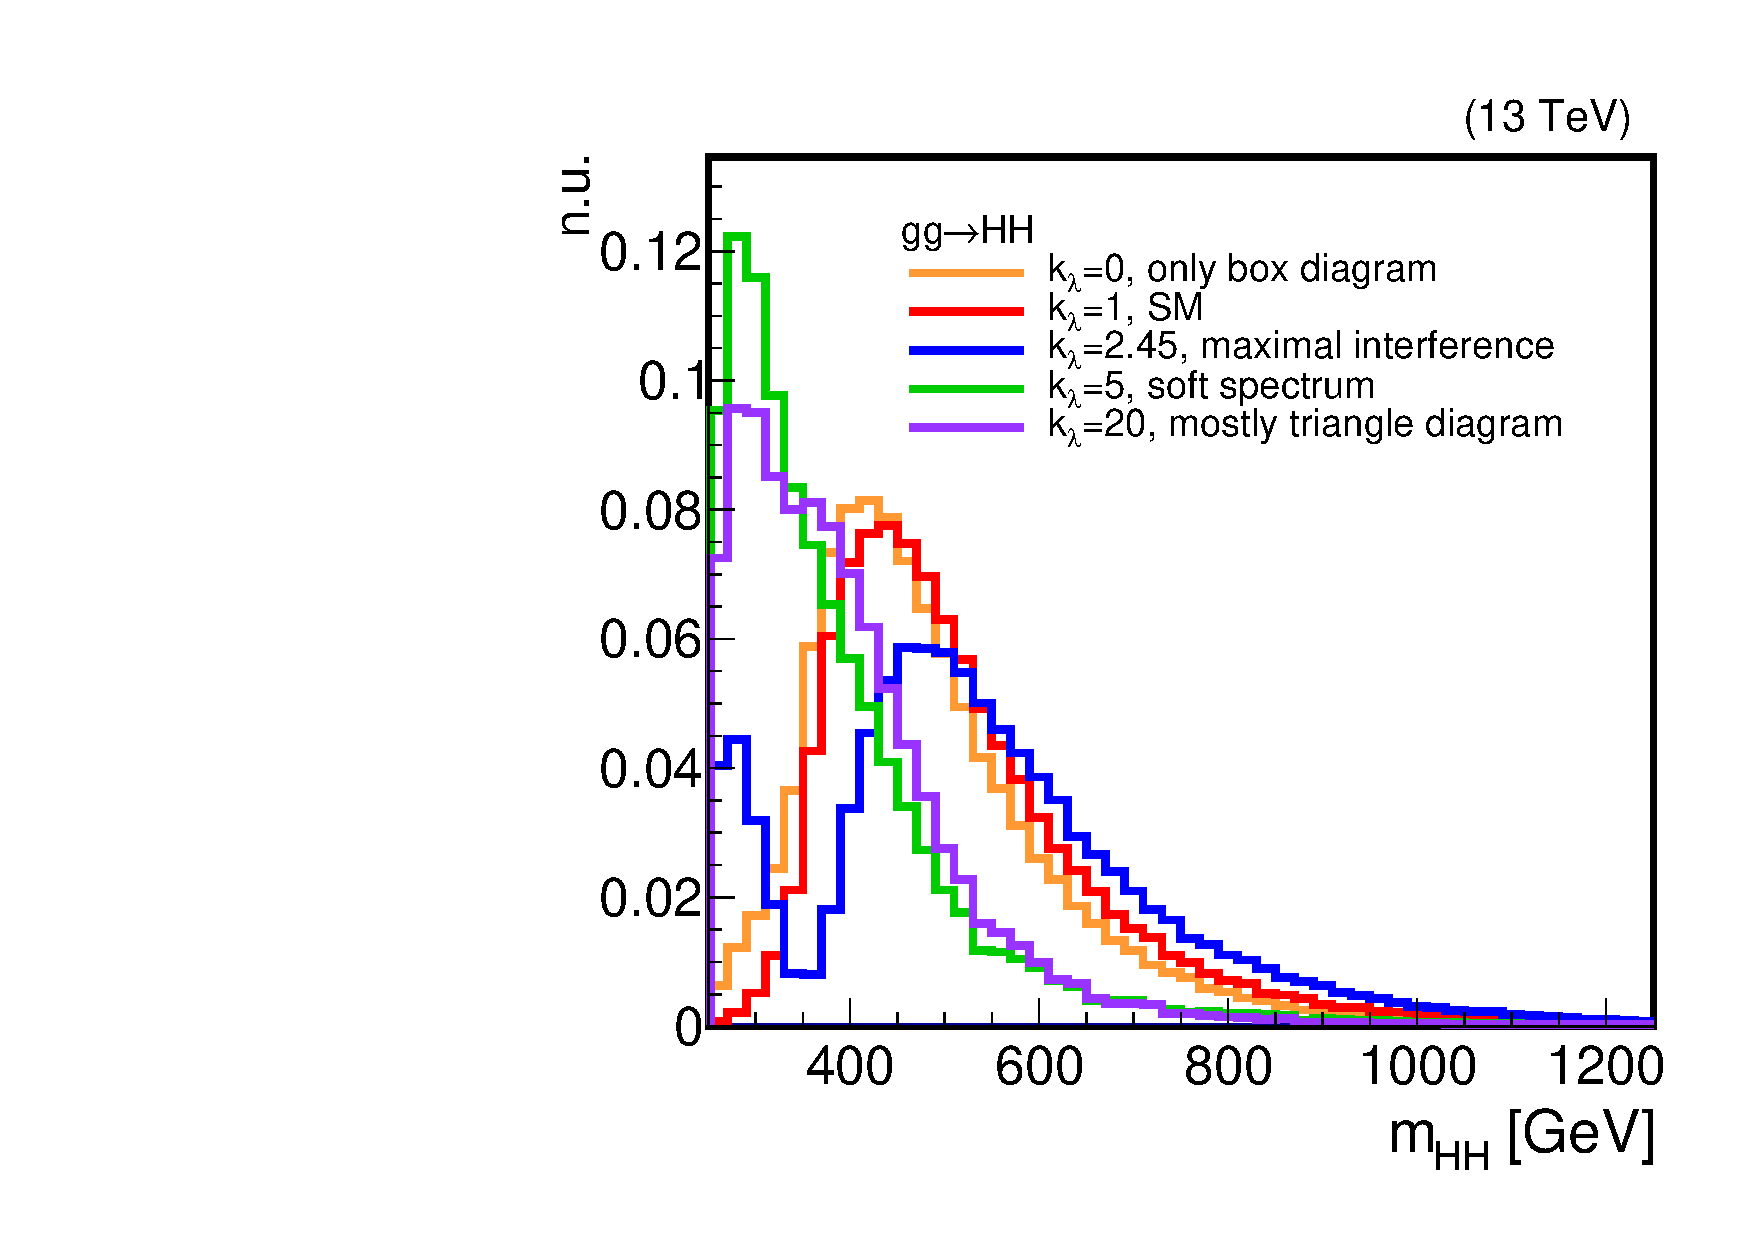
\includegraphics[width=0.50\textwidth]{Figures/HiggsPairProduction/h_gen_hh_m_ggf.pdf}}
\subfloat[]{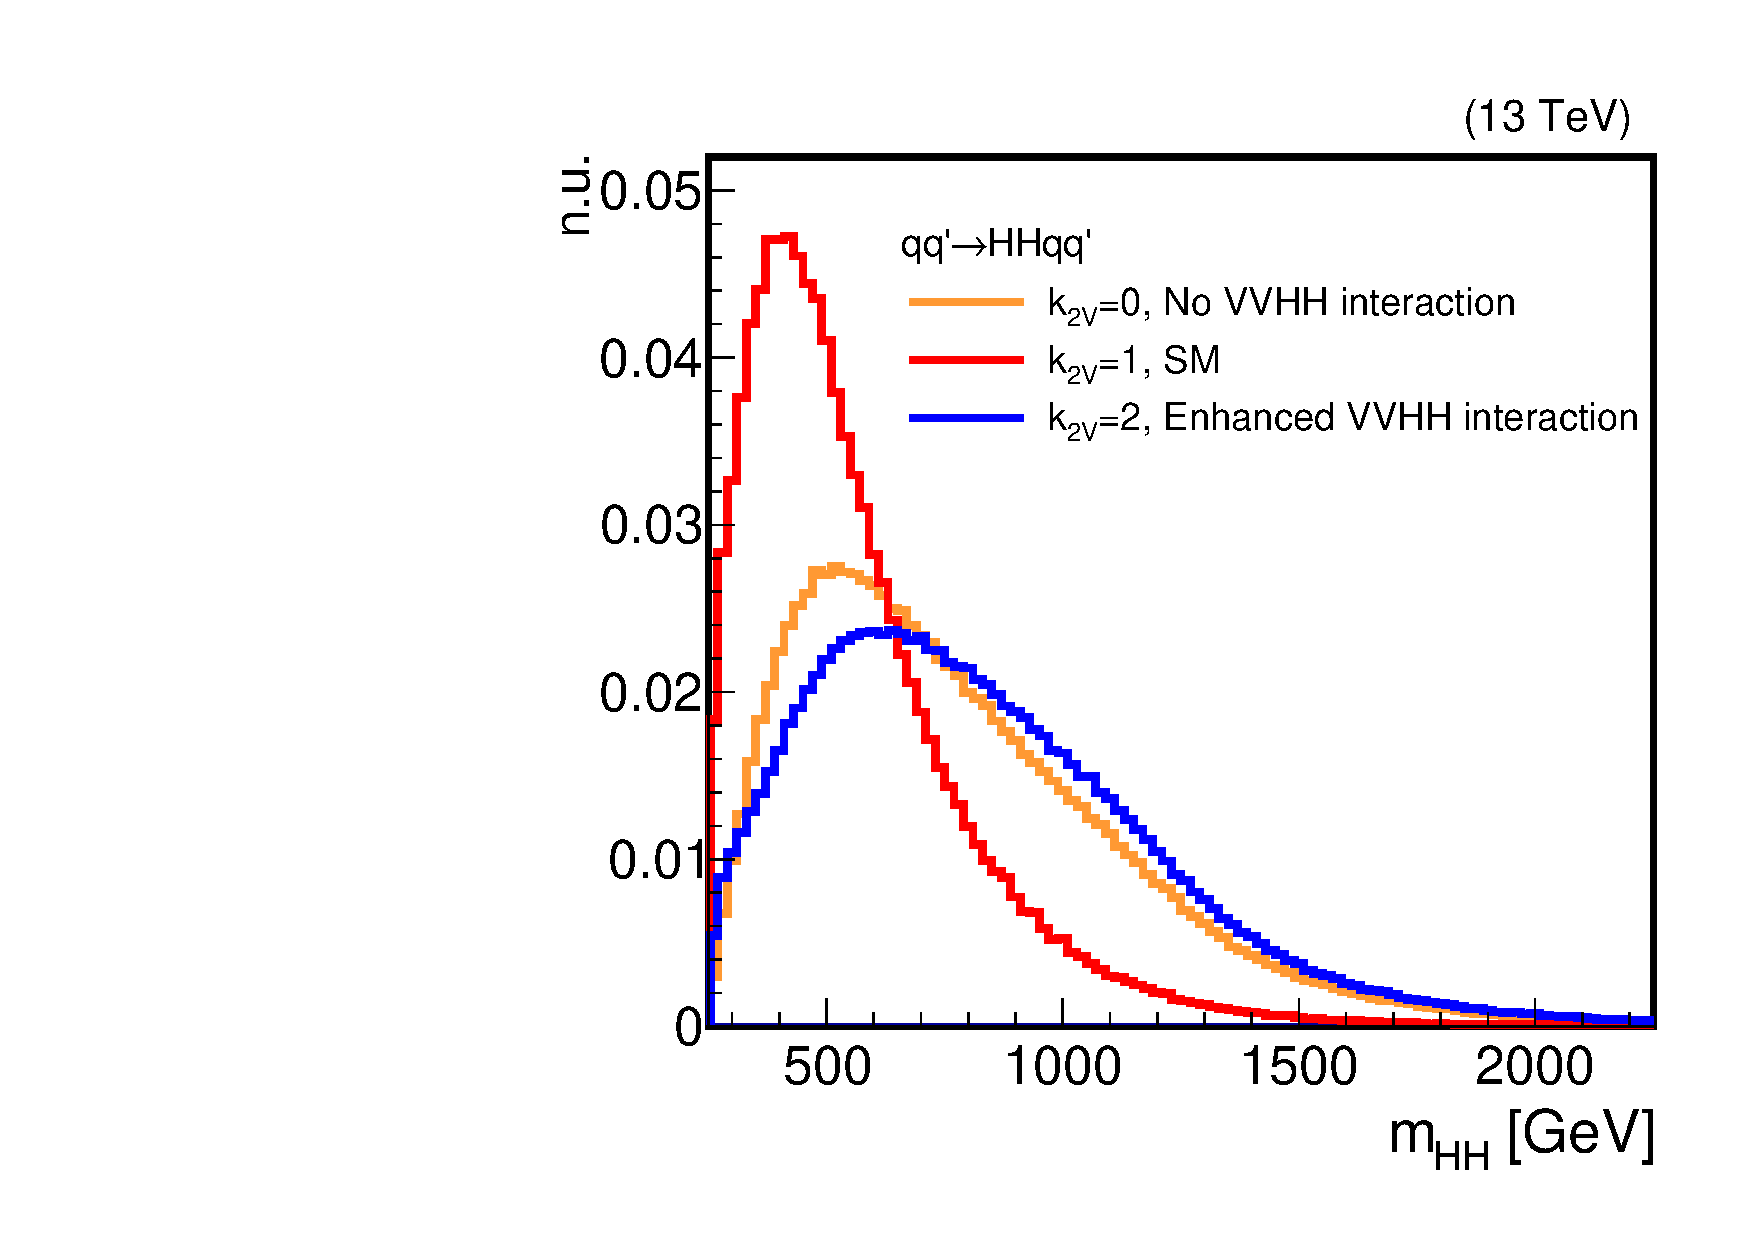
\includegraphics[width=0.50\textwidth]{Figures/HiggsPairProduction/h_gen_hh_m_vbf.pdf}}
\caption[Normalized Higgs boson pair invariant mass for different values of the coupling modifiers]{Normalized Higgs boson pair invariant mass for different values of the coupling modifiers: A) $\mathrm{\kappa_{\lambda}}$ variations in the ggF mode, and B) $\mathrm{\kappa_{2V}}$ in the VBF mode. Other Higgs couplings are set to their SM values.}
\label{fig:mhhvariation}
\end{figure}

A generalization of the BSM effects on the ggF HH production is achieved in the context of an effective field theory (EFT), where the SM Lagrangian (dimension$\leq 4$) is extended with new terms associated to dimension-6 operators~\cite{Goertz:2014qta}. The effects of these new operators represent modifications of the SM $\mathrm{y_{t}}$ and $\mathrm{\lambda_{HHH}}$ couplings with strength $\mathrm{\kappa_{\lambda}}$ and $\mathrm{\kappa_{t}=y_{t}/y_{t}^{SM}}$, and three new vertices associated to contact interactions gHH, ggHH and ttHH with coupling strengths denoted as $\mathrm{c_{g}}$, $\mathrm{c_{2g}}$ and $\mathrm{c_{2}}$, respectively. Figure~\ref{fig:cinteractions} illustrates the LO diagrams of the three EFT contact interactions. The EFT NLO accuracy model is presented in Ref.~\cite{Buchalla:2018yce}. 

\begin{figure}[htp!]
\centering
\captionsetup[subfigure]{justification=centering}
\subfloat[]{\centering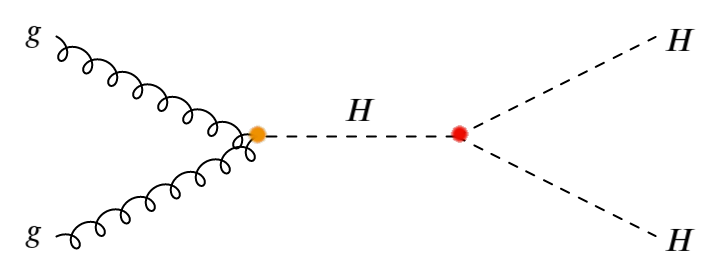
\includegraphics[width=0.35\textwidth]{Figures/HiggsPairProduction/cg.png}}
\subfloat[]{\centering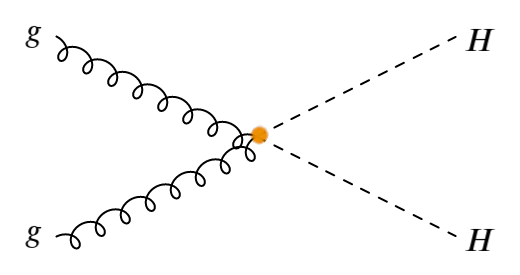
\includegraphics[width=0.29\textwidth]{Figures/HiggsPairProduction/c2g.png}}
\subfloat[]{\centering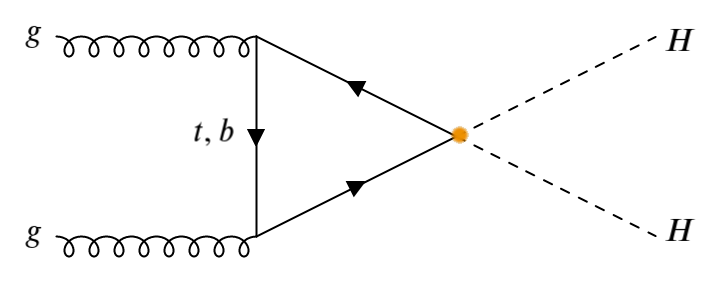
\includegraphics[width=0.35\textwidth]{Figures/HiggsPairProduction/c2.png}}
\caption[Leading order diagrams of contact interactions]{Leading order diagrams of contact interactions: A) gHH, B) ggHH and C) ttHH. The orange (red) circle represents the vertices absent in the SM (Higgs self-coupling).}
\label{fig:cinteractions}
\end{figure}

Given that is not feasible to experimentally study all possible combinations of the five EFT couplings, 12 shape benchmarks are chosen to target characteristic kinematic properties of large regions of the five-dimensional phase space by the clustering method presented in Ref.~\cite{Carvalho:2015ttv}. The coupling combination of the benchmarks are listed in Table~\ref{tab:eftcouplings} and their $\mathrm{m_{HH}}$ shapes are illustrated in Figure~\ref{fig:eftshapes}. Note that the softest spectrum corresponds to benchmark 7, whereas the hardest spectrum corresponds to benchmark 2. 

\begin{figure}[ht]
\centering
\captionsetup[subfigure]{justification=centering}
\subfloat[]{\centering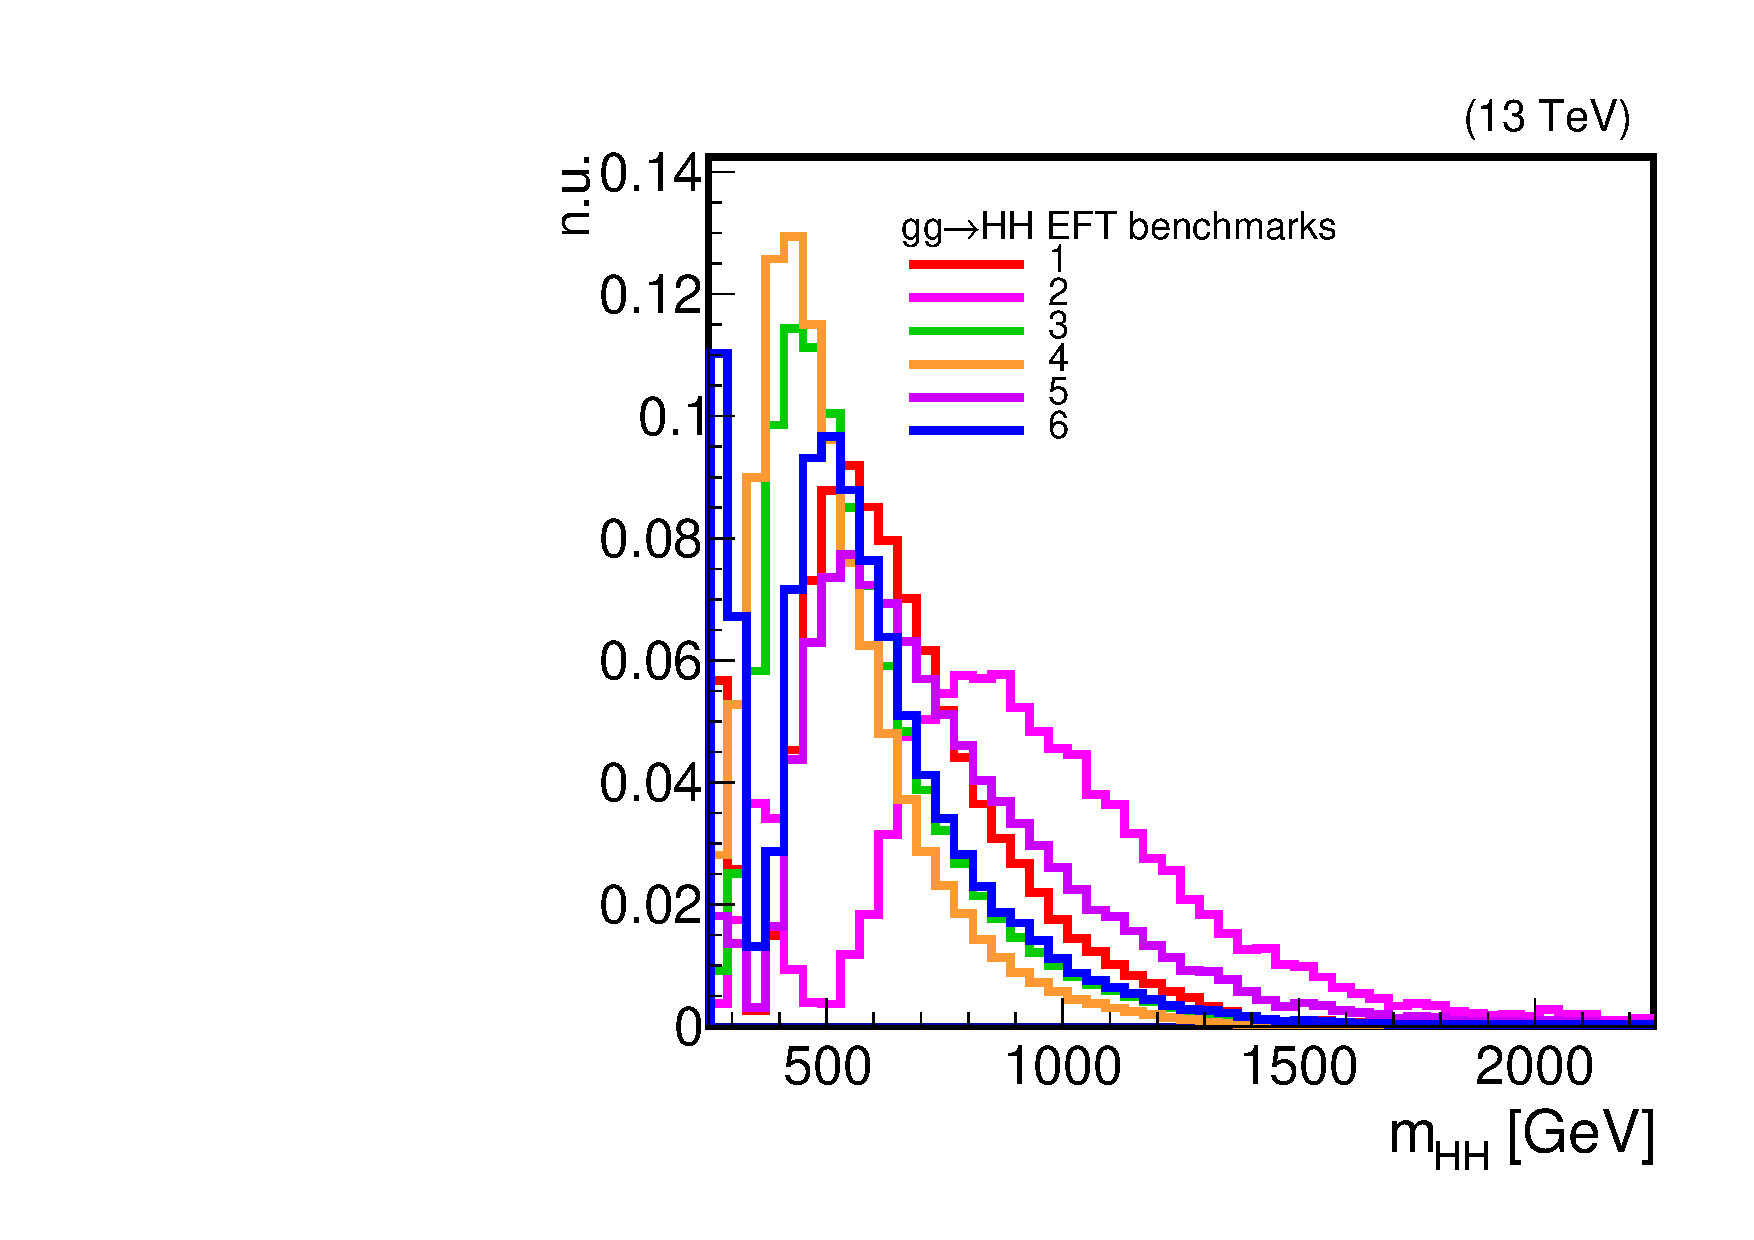
\includegraphics[width=0.42\textwidth]{Figures/HiggsPairProduction/h_gen_hh_m_eft1.pdf}}
\subfloat[]{\centering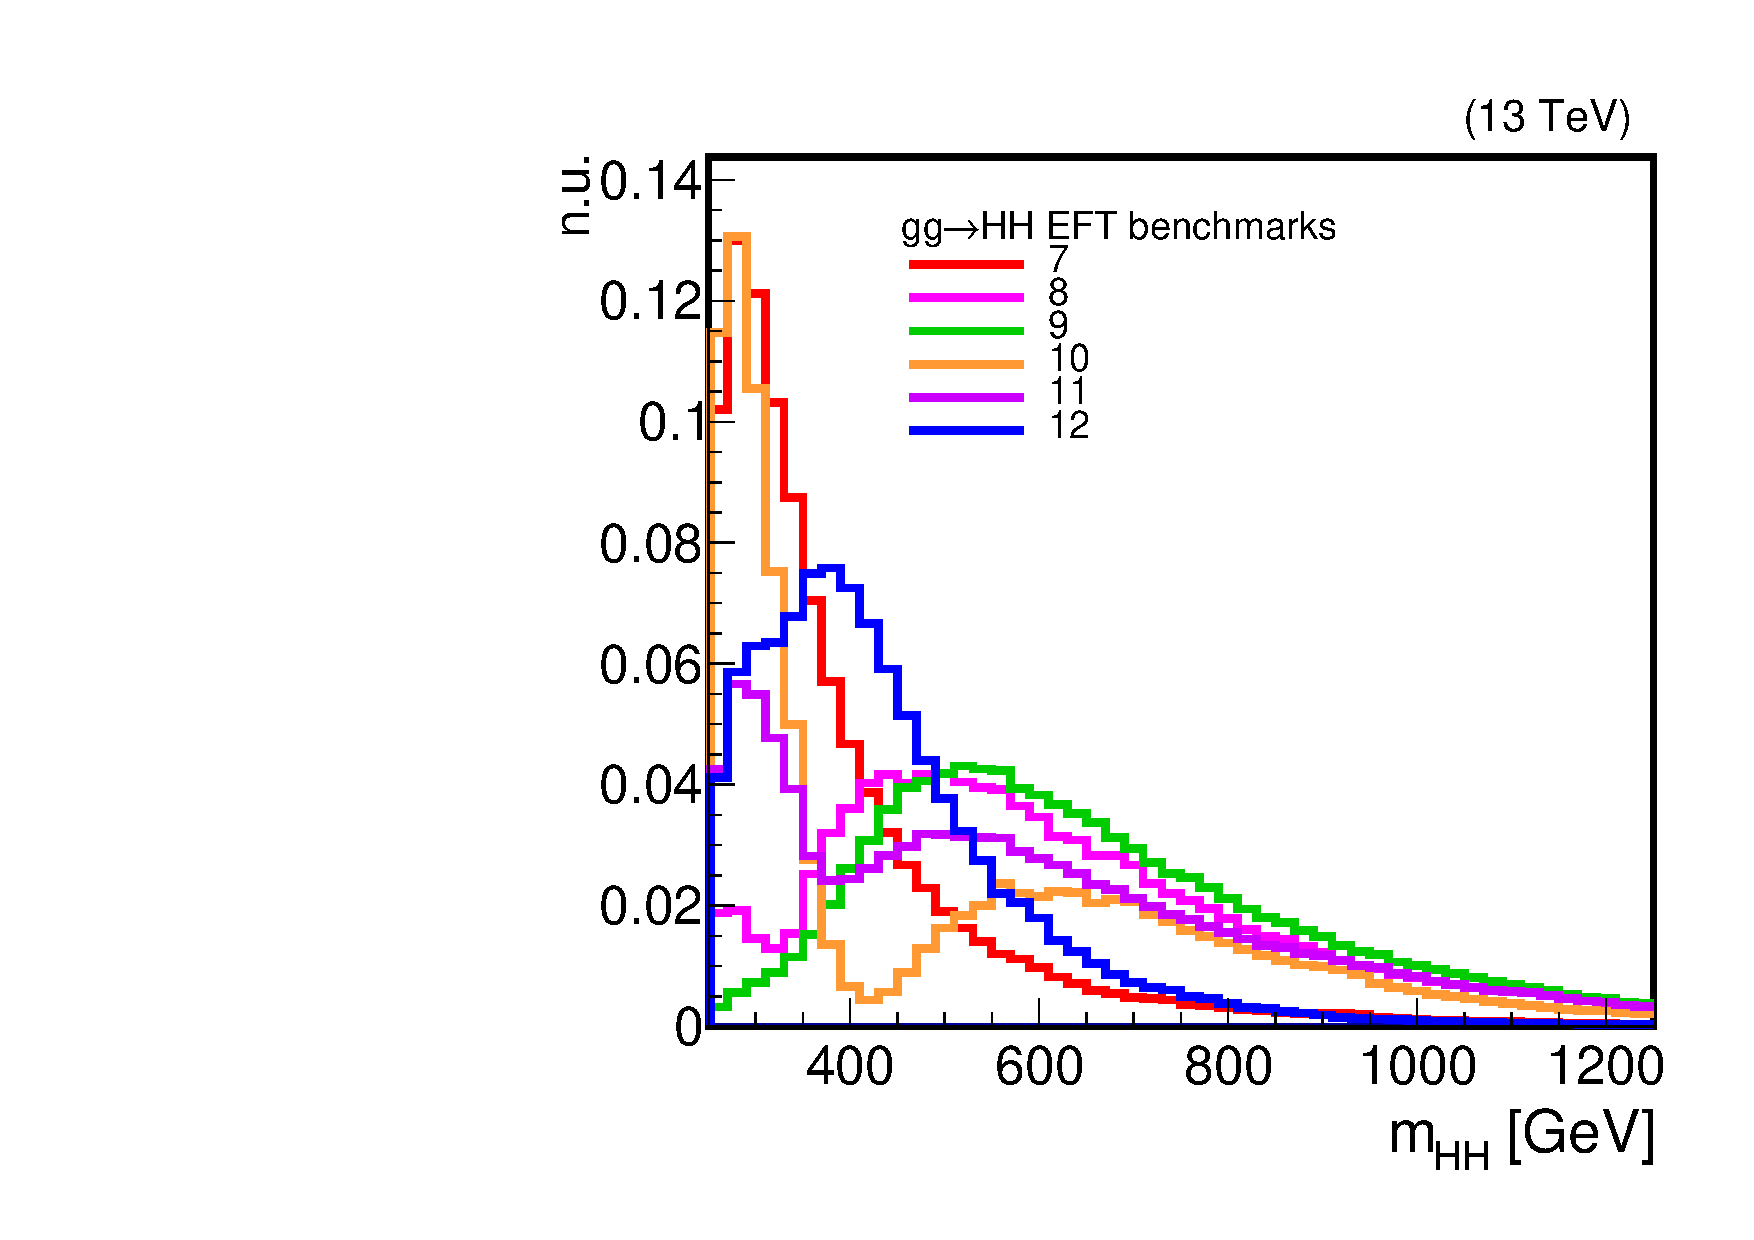
\includegraphics[width=0.42\textwidth]{Figures/HiggsPairProduction/h_gen_hh_m_eft2.pdf}}
\caption{Higgs boson pair invariant mass distribution for different leading order effective field theory (EFT) shape benchmarks: A) Nodes 1 to 6, and B) Nodes 7 to 12.}
\label{fig:eftshapes}
\end{figure}

\begin{table}[ht]
\centering
\caption[Effective field theory benchmarks for LHC searches for non-resonant Higgs boson pair production]{\label{tab:eftcouplings} Effective field theory benchmarks for LHC searches for non-resonant Higgs boson pair production via the gluon-fusion mode~\cite{Carvalho:2015ttv}.}
\begin{tabularx}{\textwidth}{XXXXXX}
\hline
Benchmark  & $\mathrm{\kappa_{\lambda}}$ &  $\mathrm{\kappa_{t}}$ &   $\mathrm{c_{2}}$ & $\mathrm{c_{g}}$  & $\mathrm{c_{g}}$ \\
\hline
1   &7.5   & 1.0  & -1.0 &  0.0 & 0.0  \\[0pt]
2   &1.0   & 1.0  &  0.5 & -0.8 & 0.6  \\[0pt]
3   &1.0   & 1.0  & -1.5 &  0.0 &-0.8  \\[0pt]
4   &-3.5  & 1.5  & -3.0 &  0.0 & 0.0  \\[0pt]
5   &1.0   & 1.0  &  0.0 &  0.8 &-1.0  \\[0pt]
6   &2.4   & 1.0  &  0.0 &  0.2 &-0.2  \\[0pt]
7   &5.0   & 1.0  &  0.0 &  0.2 &-0.2  \\[0pt]
8   &15.0  & 1.0  &  0.0 & -1.0 & 1.0  \\[0pt]
9   &1.0   & 1.0  &  1.0 & -0.6 & 0.6  \\[0pt]
10  &10.0  & 1.5  & -1.0 &  0.0 & 0.0  \\[0pt]
11  &2.4   & 1.0  &  0.0 &  1.0 &-1.0  \\[0pt]
12  &15.0  & 1.0  &  1.0 &  0.0 & 0.0  \\[0pt]
\hline
\end{tabularx}
\end{table}


\clearpage

\section{Searches for Higgs Boson Pair Production}
This section reviews the phenomenology and experimental aspects of the ongoing HH program at the LHC. First, the HH decay channels and their properties are discussed. Then, the results of the searches performed using LHC pp collision data are summarized. It ends with the most recent projections for the SM HH production at the High Luminosity LHC (HL-LHC), which were prepared in the context of the European Strategy for Particle Physics before the development of this dissertation~\cite{deBlas:2019rxi}.

\subsection{Decay Channels}
SM HH production is an elusive process to measure due to the low expected rates at the LHC. However, as mentioned before, rates and kinematics can be modified by BSM effects and potentially discovered with the current datasets. The HH signature has a rich variety of decay channels with different branching fractions depending on the two Higgs boson decays as seen in Figure~\ref{fig:hhbr}. The $\mathrm{b\overline{b}b\overline{b}}$ is the dominant decay channel with $\sim33\%$ branching fraction. Decay channels with at least one $\mathrm{H\rightarrow~bb}$ are used in searches to maintain a sizeable branching fraction.

\begin{figure}[ht!]
\centering
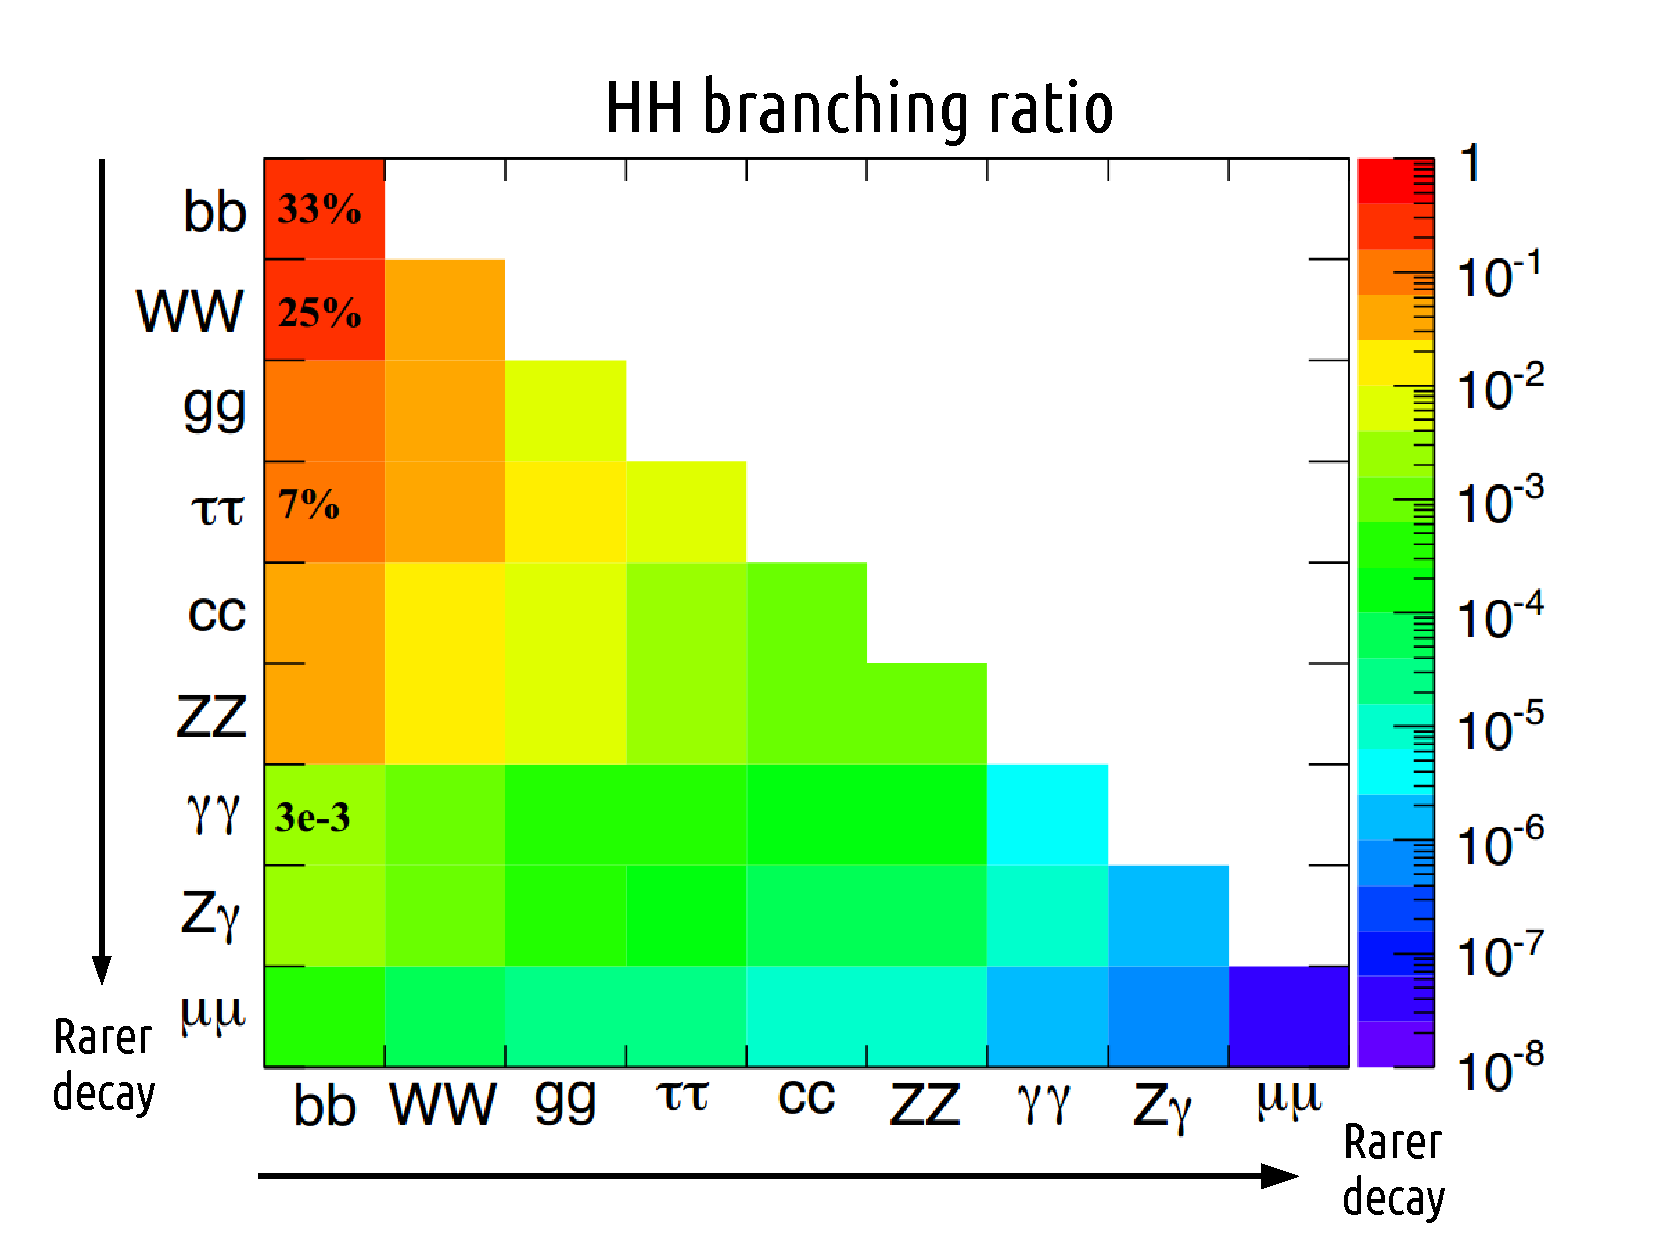
\includegraphics[width=0.63\textwidth]{Figures/HiggsPairProduction/brhh.pdf}
\caption[Higgs boson pair branching fractions assuming a Higgs mass $\mathrm{m_{H}=125~GeV}$]{Higgs boson pair branching fractions assuming a Higgs mass $\mathrm{m_{H}=125~GeV}$. The Higgs decays considered in the figure are: two bottom quarks ($\mathrm{b\overline{b}}$), two W bosons ($W^{+}W^{-}$), two gluons (gg), two tau leptons ($\tau^{+}\tau^{-}$), two charm quarks (cc), two Z bosons (ZZ), two photons ($\gamma\gamma$), a Z boson and a photon (Z$\gamma$), and two muons ($\mu\mu$).}
\label{fig:hhbr}
\end{figure}

\subsection{Experimental Status at the LHC}
The LHC has a broad experimental program exploring resonant and non-resonant HH production in multiple channels and production modes. The first results were obtained analyzing the Run-1 collision data at 8 TeV, corresponding to around 20$\mathrm{fb^{-1}}$ of integrated luminosity. ATLAS (CMS) studied the gluon fusion HH production in the  $\mathrm{b\overline{b}\gamma\gamma}$, $\mathrm{b\overline{b}\tau^{+}\tau^{-}}$, $\mathrm{b\overline{b}b\overline{b}}$ and $\gamma\gamma~W^{+}W^{-}$ ($\mathrm{b\overline{b}\gamma\gamma}$, $\mathrm{b\overline{b}\tau^{+}\tau^{-}}$ and $\mathrm{b\overline{b}b\overline{b}}$). The Run-1 ATLAS (CMS) observed combined upper limits on the SM-like HH production cross section corresponds to 70 (43) times the SM prediction, respectively. Other results in the context of BSM $\kappa_{\lambda}$ couplings and resonances were presented, but no significant excess of signal was observed~\cite{atlashhrun1comb,cmshhrun1comb}.

At the present time, CMS and ATLAS experts are exploring searches with more production modes and new decay channels by analyzing the full Run-2 dataset collected at 13 TeV. While those results are being finished, both experiments already released a very comprehensive study of direct searches via the ggF mode by combining the results obtained in several channels using partial Run-2 dataset~\cite{atlascomb,cmscomb}. The ATLAS (CMS) dataset was collected during the 2015-2016 (2016) operations with an integrated luminosity of 27.1--36.1 (35.9) $\mathrm{fb^{-1}}$. The ATLAS (CMS) channels used in the combination are the following: $\mathrm{b\overline{b}\gamma\gamma}$~\cite{bbggatlas}, $\mathrm{b\overline{b}\tau^{+}\tau^{-}}$~\cite{bbttatlas1}, $\mathrm{b\overline{b}b\overline{b}}$~\cite{bbbbatlas}, $\mathrm{W^{+}W^{-}W^{+}W^{-}}$~\cite{atlaswwww} and $\gamma\gamma\mathrm{W^{+}W^{-}}$~\cite{atlasggww} ($\mathrm{b\overline{b}b\overline{b}}$ boosted~\cite{bbbbcmsr2} and resolved~\cite{bbbbcmsnr,bbbbcmsr1}, $\mathrm{b\overline{b}}\gamma\gamma$~\cite{bbggcms}, $\mathrm{b\overline{b}}\tau^{+}\tau^{-}$~\cite{bbttcms1,bbttcms2}, $\mathrm{b\overline{b}VV}$~\cite{cmsbbvv}). In addition, both experiments studied indirect $\kappa_{\lambda}$ constraints from single Higgs searches~\cite{cmsrun2mes,atlasindirecthh}.

The ATLAS (CMS) combination set an observed limit on the SM production cross section at 6.9 (22) times the SM prediction. The observed allowed $\kappa_{\lambda}$ interval at 95\% CL ranges from -5.0 (-11.8) to 12.0 (18.8). Results on EFT benchmarks were also presented. Furthermore, both experiments presented results on resonant searches for new particles with Spin-0 and Spin-2 in the mass range between 250 GeV and 3 TeV. However, no statistically significant excess of resonant events were observed, and 95\% CL limits on the production cross section of new resonances decaying into Higgs pairs were provided. In addition, the ATLAS (CMS) results from single Higgs searches presented the 95\% CL allowed $\kappa_{\lambda}$ interval from -3.2 (-3.5) to 11.9 (14.5).

Excluding the results of this dissertation, several Run-2 HH non-resonant analyses have been performed. The ATLAS experiment has presented the study of the ggF production mode in the $\mathrm{b\overline{b}\gamma\gamma}$~\cite{atlasfullrun2bbgg}, $\mathrm{b\overline{b}\tau^{+}\tau^{-}}$~\cite{atlasrun2bbtt},  and $\mathrm{b\overline{b}W^{+}W^{-}(\ell\nu\ell\nu)}$~\cite{atlasfullrun2bbwwdilep} channels, whereas the CMS experiment has explored the same mode in the $\mathrm{b\overline{b}\gamma\gamma}$~\cite{cmsfullrun2bbgg} and $\mathrm{b\overline{b}ZZ(4\ell)}$~\cite{cmsbbzz4l} channels. Moreover, the VBF production mode has been explored by the ATLAS experiment in the $\mathrm{b\overline{b}b\overline{b}}$~\cite{atlasfullrun2vbf4b}, whereas CMS experiment has done it in the $\mathrm{b\overline{b}\gamma\gamma}$~\cite{cmsfullrun2bbgg} channel, and the $\mathrm{b\overline{b}b\overline{b}}$ channel studying highly Lorentz-boosted Higgs bosons~\cite{cmsrun2boostedbbbb}.  Once the main decay channels are analyzed, then a full Run-2 HH combination will be performed. In addition, full Run-2 resonant searches have also been performed in ATLAS~\cite{atlasfullrun2bbgg,atlasrun2bbtt,atlasfullrun2vbf4b} and CMS~\cite{cmsrun2resboostbbbb,cmsrun2resboostbbww}. 

The best LHC results on non-resonant HH production are obtained from the currently finalized full Run-2 analyses. From the ATLAS combination of the results of the $\mathrm{b\overline{b}\gamma\gamma}$ and $\mathrm{b\overline{b}\tau^{+}\tau^{-}}$ channels, the current observed limit on the SM-like HH production cross section is 3.1 times the SM expectation, and the observed allowed $\kappa_{\lambda}$ interval at 95\% CL is from -1.0 to 6.6 as presented in Figure~\ref{fig:hhbestresults} A)~\cite{ATLAS-CONF-2021-052}. Furthermore, the current observed limit on VBF production cross section is 225 times the SM prediction by the CMS search in the $\mathrm{b\overline{b}\gamma\gamma}$ channel. Finally, the observed allowed interval of the $\kappa_{2V}$ modifier is from 0.6 to 1.4, corresponding to the search in the $\mathrm{b\overline{b}b\overline{b}}$ channel with highly Lorentz-boosted Higgs bosons (illustrated in Figure~\ref{fig:hhbestresults}~B))~\cite{cmsrun2boostedbbbb}.

The search sensitivity of the HH searches depends on the rates (production cross section and branching ratio), selection efficiencies, level of background contamination and mass resolution. The HH signal is reconstructed by the ATLAS and detectors from objects associated to the final state particles. These objects are b-quark hadronic jets (b) or `b-jets', light-quark jets (j), hadronic or leptonic $\tau$ leptons, muons and electrons ($\ell$), photons ($\gamma$), and missing transverse energy (MET) if neutrinos ($\nu$) are present. As the quality of the object reconstruction has a direct impact on the HH signal identification, ATLAS and CMS have developed algorithms to improve it. For instance, there are dedicated jet identification algorithms based on machine learning to improve the reconstruction of the $\mathrm{H\rightarrow~b\overline{b}}$ decay from two small-radius b-jets or a large-radius jet (if H has a large Lorentz boost)~in CMS~\cite{cmsbtag1,cmsbtag2} and ATLAS~\cite{atlasbtag1,atlasbtag2}. Moreover, there are multivariate regression algorithms to correct the reconstructed b-jet energy from the unmeasured energy associated neutrinos inside the b-jet from semileptonic B hadron decays~(e.g. see Ref.\cite{cmsbreg}).

\begin{figure}[ht!]
\centering
\captionsetup[subfigure]{justification=centering}
\subfloat[]{\centering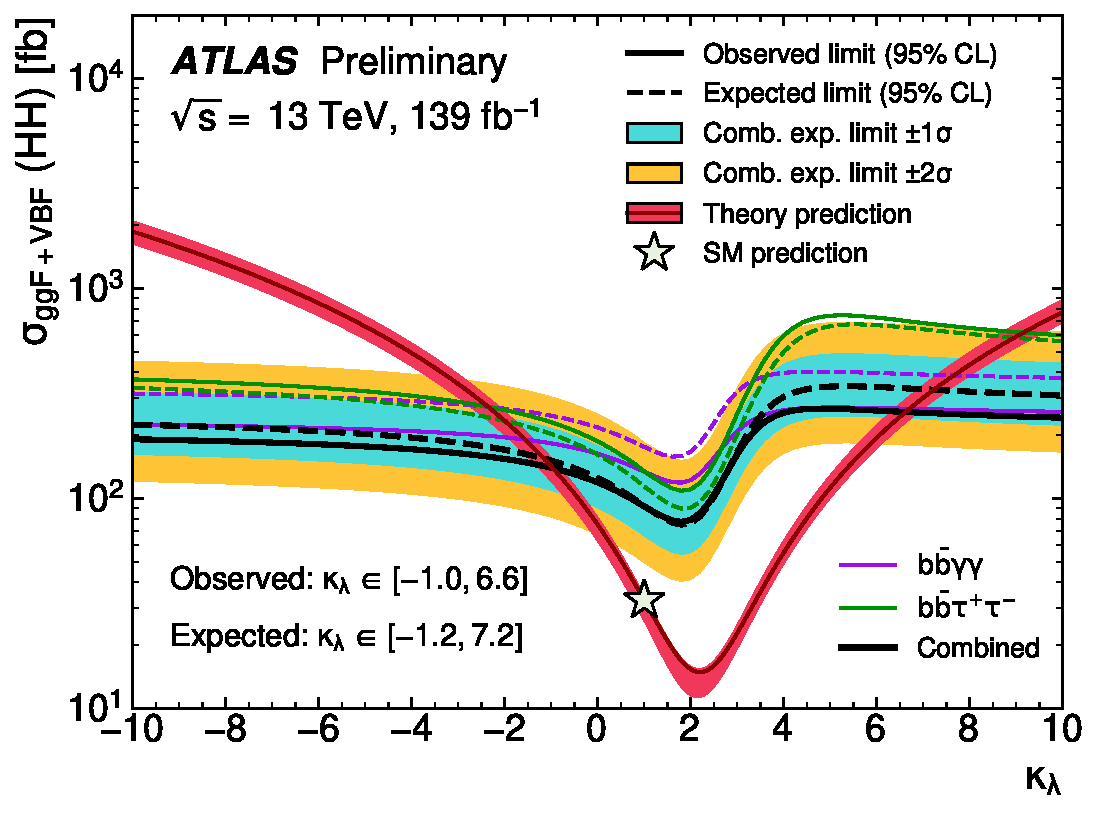
\includegraphics[width=0.45\textwidth]{Figures/HiggsPairProduction/bestatlashh.pdf}}
\subfloat[]{\centering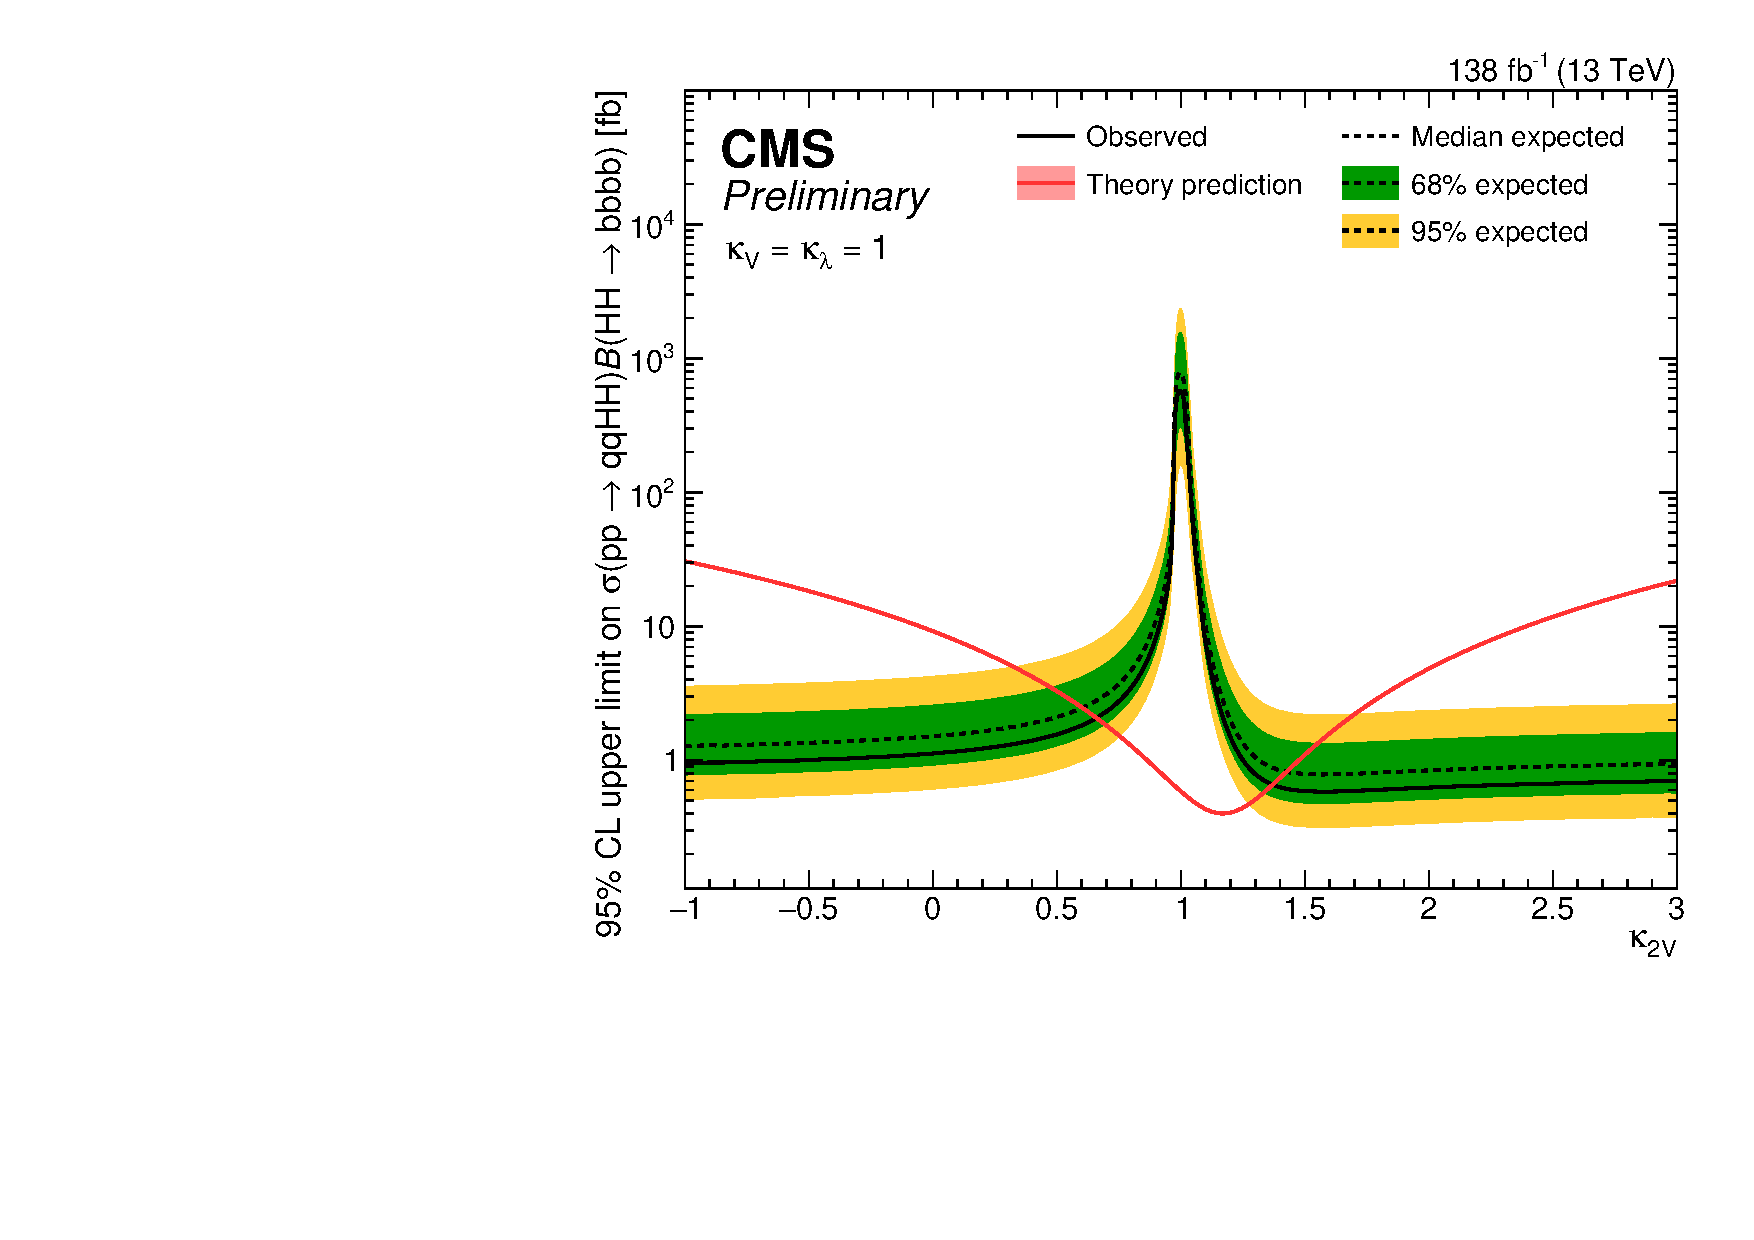
\includegraphics[width=0.42\textwidth]{Figures/HiggsPairProduction/bestk2vresult.pdf}}
\caption[95\% CL observed and expected upper limits on the Higgs boson pair production cross section as function of the coupling modifiers]{95 \% CL observed and expected upper limits on the Higgs boson pair production cross section as function of the coupling modifiers. A) Gluon fusion and vector boson fusion production cross section as a function of $\kappa_{\lambda}$~\cite{ATLAS-CONF-2021-052}, B) Vector boson fusion cross section as a function of $\kappa_{2V}$~\cite{cmsrun2boostedbbbb}.}
\label{fig:hhbestresults}
\end{figure}

There are three crucial HH decay channels based on the experience gained in the Run-1 and 2016 analyses: $\mathrm{b\overline{b}\gamma\gamma}$, $\mathrm{b\overline{b}\tau^{+}\tau^{-}}$ and $\mathrm{b\overline{b}b\overline{b}}$. Their properties and experimental aspects are summarized in the following points:
\begin{itemize}
\item $\mathrm{b\overline{b}\gamma\gamma}$: This channel has a small branching ratio ($\sim0.3\%$) but a resonant signature over smoothly falling small background from multi-jet + photons ($\mathrm{N\gamma + jets,~N=1,2}$) processes. There is also a background contribution from single Higgs production ($\mathrm{H\rightarrow\gamma\gamma + jets}$) production. It is very sensitive for searches at low $\mathrm{m_{HH}}$ mass. The observables used for signal identification are based on the reconstructed masses of the two Higgs bosons taking advantage of the excellent di-photon mass resolution, as illustrated in Figure~\ref{fig:hhsearchobservables} A).
\item $\mathrm{b\overline{b}\tau^{+}\tau^{-}}$: This decay channel has an intermediate branching ratio but challenging background from top-quark pair, Drell-Yan (Z/$\gamma$ + jets) and multi-jet production. Searches are performed using the $\mathrm{H\rightarrow~\tau^{+}\tau^{-}}$ final states with two hadronic decays ($\tau_{had}\tau_{had}$), one hadronic and one leptonic decays ($\mathrm{\tau_{had}\tau_{\ell=e,\mu}}$). The signal identification is performed using observables based on Higgs pair mass and machine learning algorithms, as seen in Figure~\ref{fig:hhsearchobservables} B).
\item $\mathrm{b\overline{b}b\overline{b}}$: This channel is the focus of this dissertation. It benefits from the largest branching fraction. However, there is an overwhelming amount of multi-jet background processes, which make it very hard to measure it. Consequently, these searches relies on the good performance of the jet flavor tagging algorithms and a precise measurement of the background from data. The signal identification discriminants are based on machine learning and the Higgs pair mass, e.g. in Figure~\ref{fig:hhsearchobservables} C). This is the most sensitive channel for searches at high $\mathrm{m_{HH}}$ mass. 
\end{itemize}

\begin{figure}[ht!]
\centering
\captionsetup[subfigure]{justification=centering}
\subfloat[]{\centering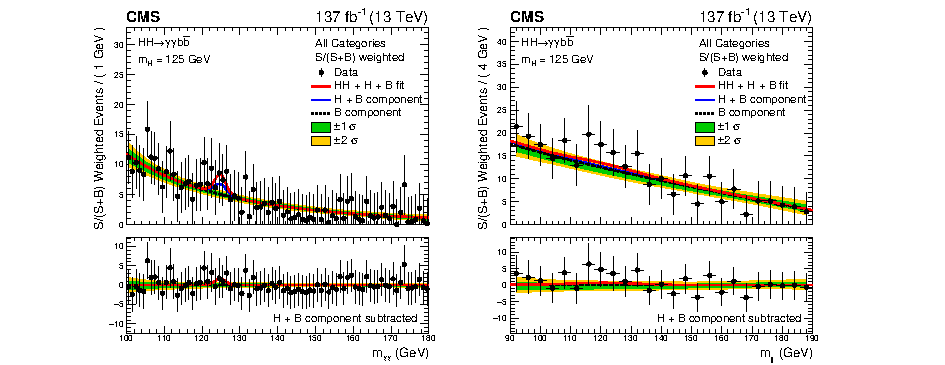
\includegraphics[width=1.0\textwidth]{Figures/HiggsPairProduction/bbggobservables.pdf}}\\
\subfloat[]{\centering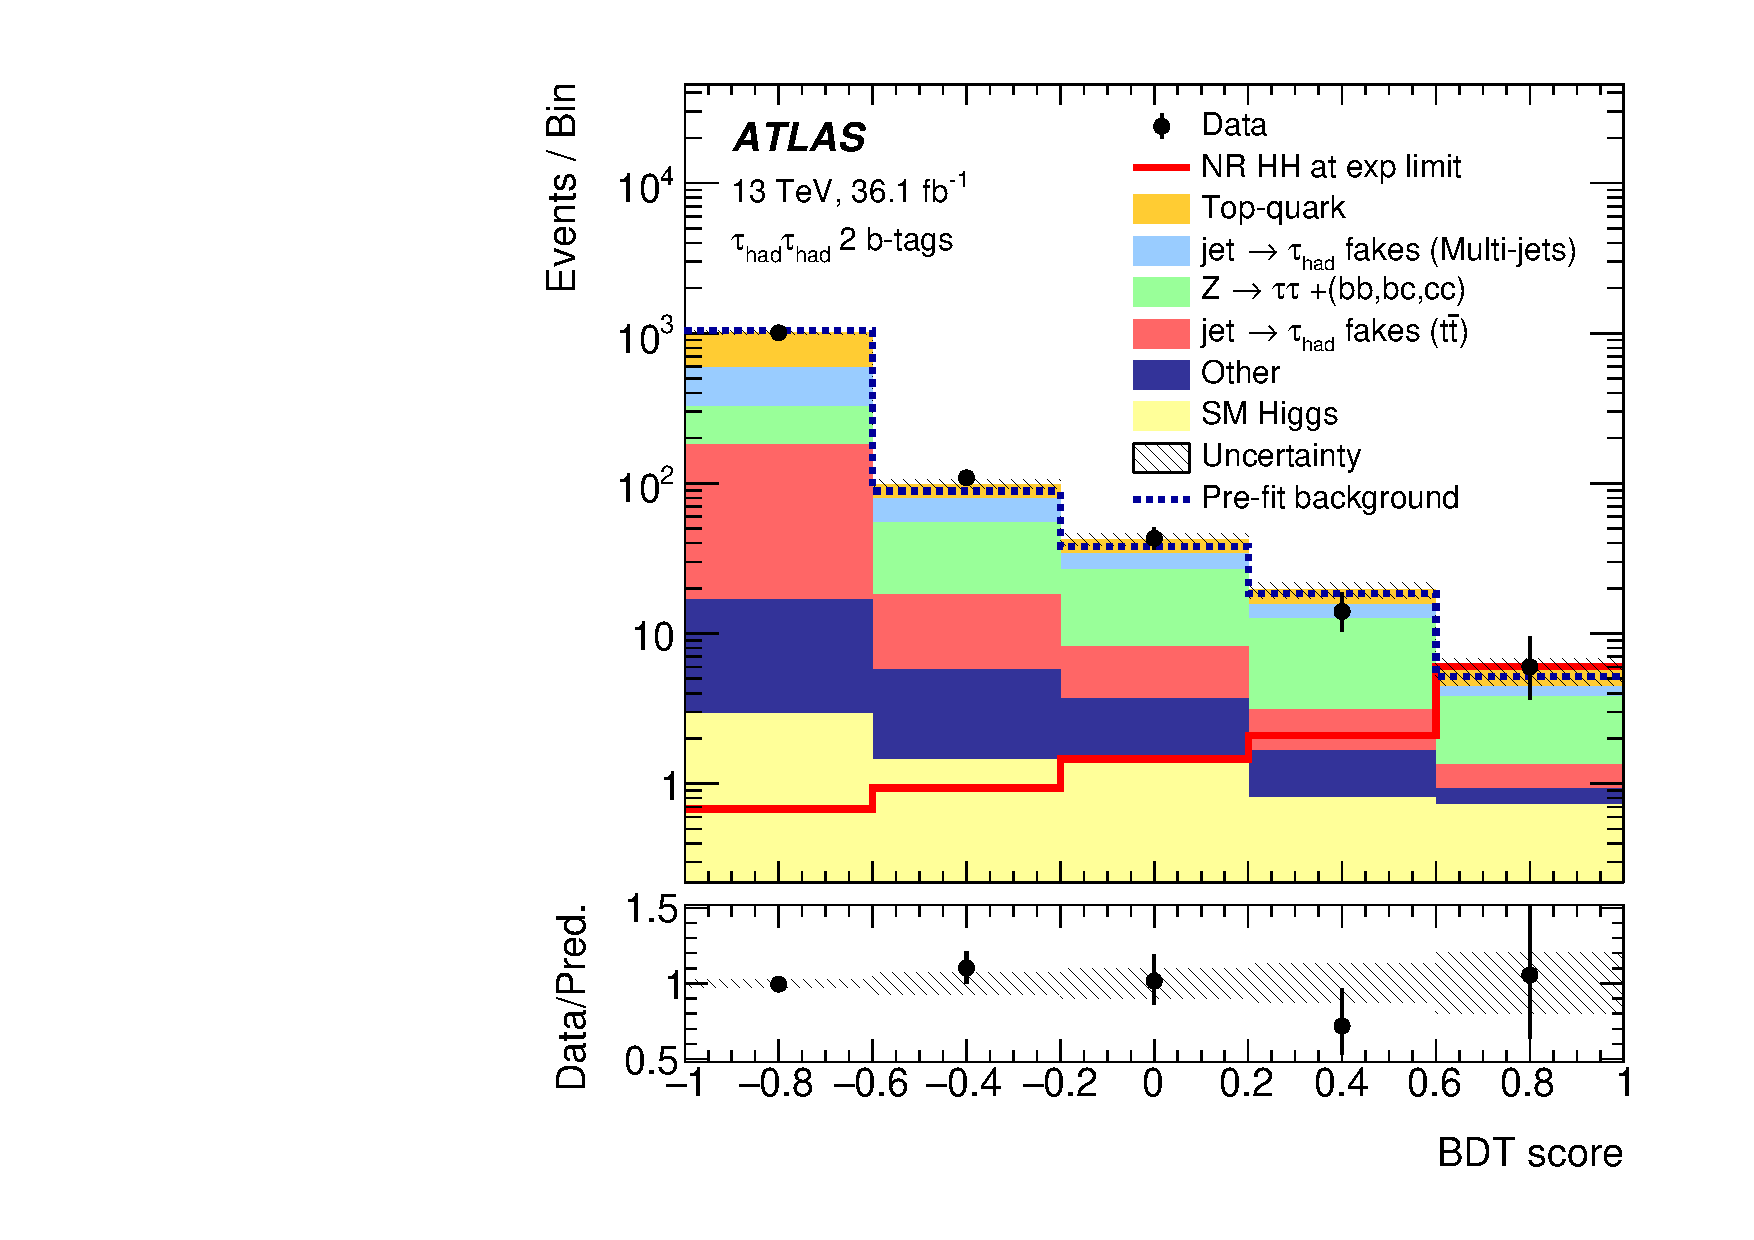
\includegraphics[width=0.40\textwidth]{Figures/HiggsPairProduction/bbtautauobservable.pdf}}
\subfloat[]{\centering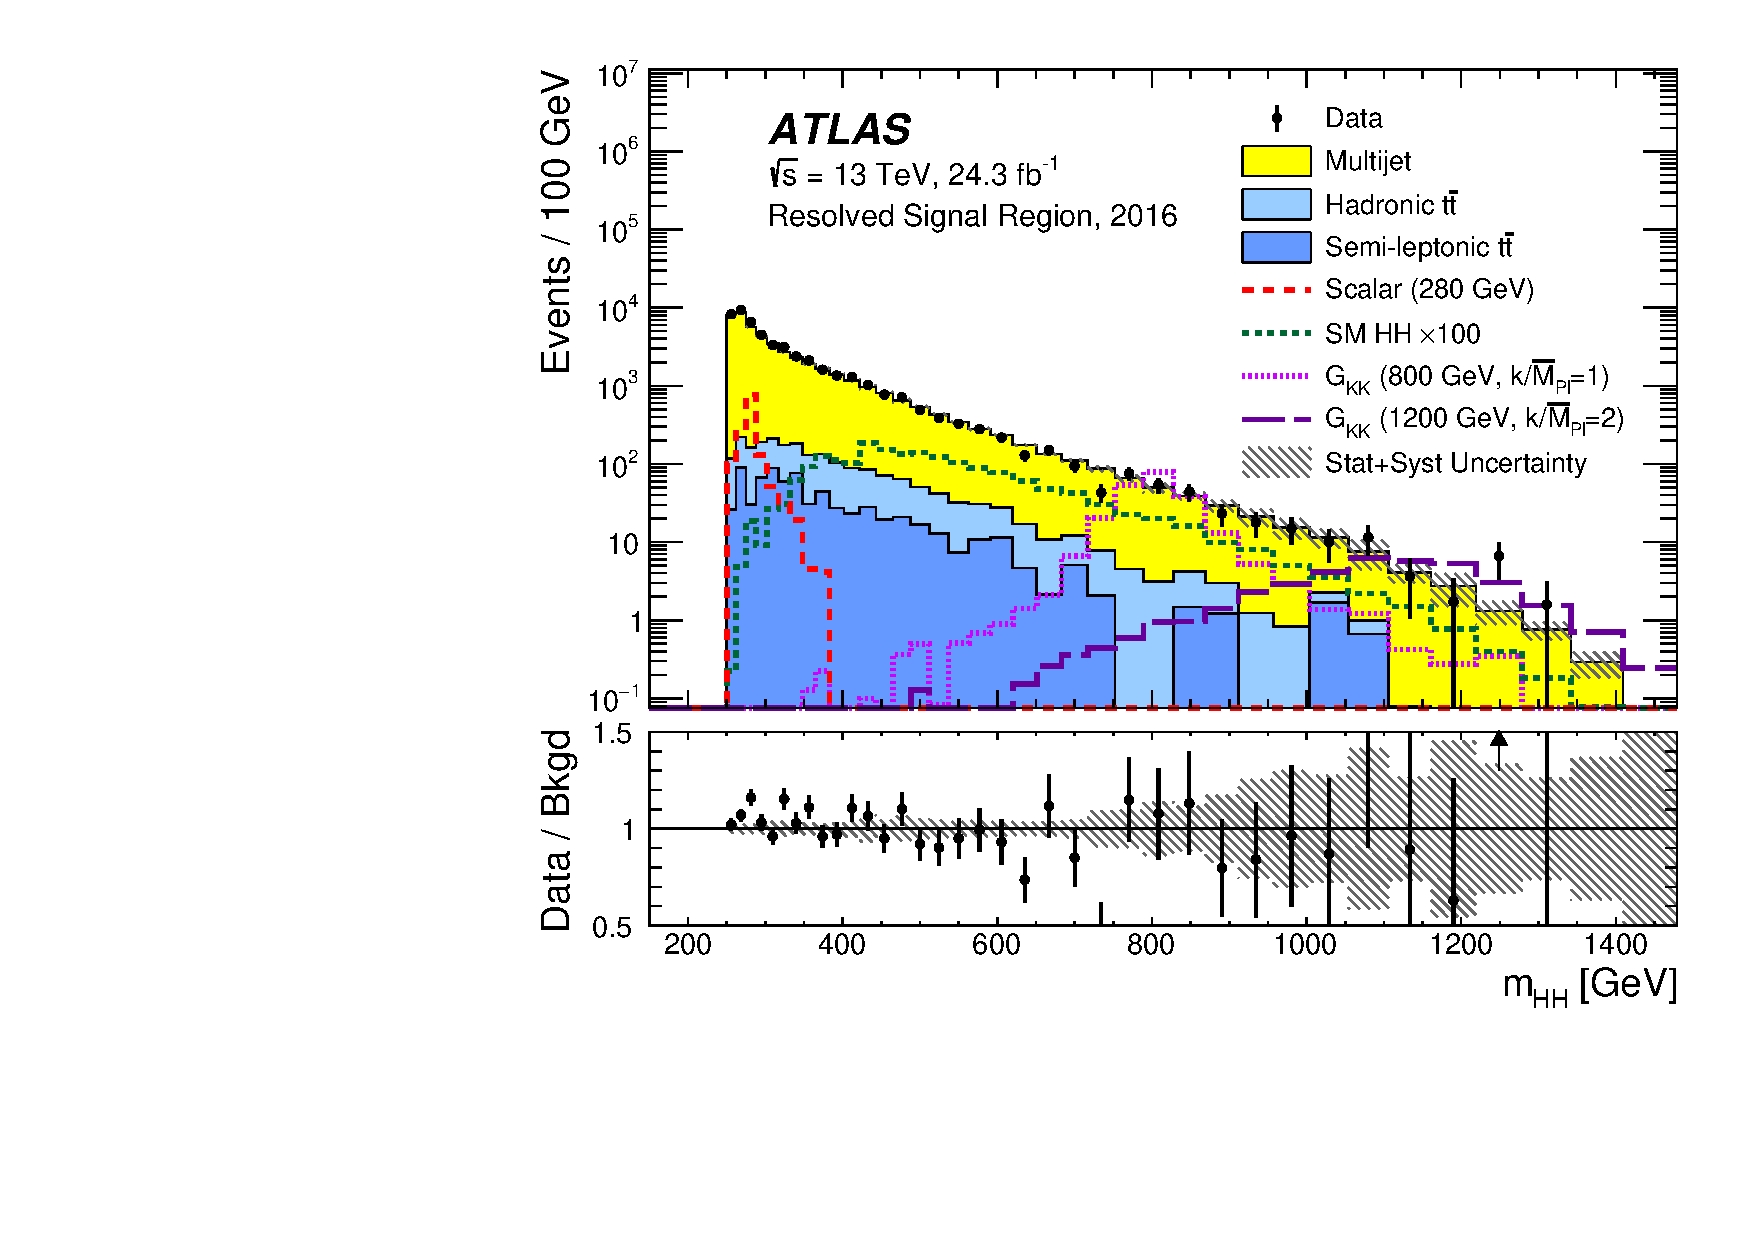
\includegraphics[width=0.46\textwidth]{Figures/HiggsPairProduction/bbbbobservable.pdf}}
\caption[Signal observables used in searches for HH production]{Signal observables used in searches for HH production. A) di-photon and bottom-quark pair distributions used in the last search for $\mathrm{HH\rightarrow~b\overline{b}\gamma\gamma}$ by CMS~\cite{cmsfullrun2bbgg}, B) Boosted decision trees (BDT) distribution used in the last search for $\mathrm{HH\rightarrow~b\overline{b}\tau^{+}\tau^{-}}$ by ATLAS~\cite{bbttatlas1}, C) Higgs boson pair mass distribution used in the last search for $\mathrm{HH\rightarrow~b\overline{b}b\overline{b}}$ by ATLAS~\cite{bbbbatlas}.}
\label{fig:hhsearchobservables}
\end{figure}

\subsection{Future Prospects at the High Luminosity LHC}
The LHC is currently under its second long shutdown (LS2) and preparing for the Run-3 data-taking program (2022-2025). Next, CMS and ATLAS will upgrade their detectors, trigger and data acquisition systems during a third long shutdown (LS3) to prepare themselves for the ultimate configuration of the LHC, the so-called High Luminosity LHC (HL-LHC). Each experiment is expected to collect a dataset of pp collisions at 14 TeV of center-of-mass energy within 10 years of the HL-LHC operation, corresponding to 3000--4000 $\mathrm{fb^{-1}}$ of integrated luminosity ($\sim20$ times more than in Run-2). More details are discussed in Chapter~\ref{chapter:apparatus}.  

The analysis of these large dataset will be crucial for a potential measurement of the SM HH production and the Higgs boson self-coupling $\mathrm{\lambda_{HHH}}$. In consequence, ATLAS and CMS experiments have already started to study what the challenges and developments needed are to reach that goal in the future. Both have presented the most recent projections of the searches for this elusive process at the HL-LHC based on the current analysis strategies on the gluon fusion mode and assuming an expected integrated luminosity of 3000 $\mathrm{fb^{-1}}$~\cite{atlasprojections,cmsprojections}. In these studies, the channels considered by ATLAS (CMS) are  $\mathrm{b\overline{b}\gamma\gamma}$, $\mathrm{b\overline{b}\tau^{+}\tau^{-}}$ and  $\mathrm{b\overline{b}b\overline{b}}$  ($\mathrm{b\overline{b}\gamma\gamma}$, $\mathrm{b\overline{b}\tau^{+}\tau^{-}}$, $\mathrm{b\overline{b}b\overline{b}}$, $\mathrm{b\overline{b}VV(\ell\ell\nu\nu)}$ and $\mathrm{b\overline{b}ZZ(4\ell)}$). In particular, the $\mathrm{b\overline{b}b\overline{b}}$ channel studies show that its main challenges will be our capability to have online triggers with high signal selection efficiency and model the multi-jet background events with high precision. 
\begin{table}[htb]
\centering
\caption[ATLAS and CMS expected significance (in standard deviation) for SM Higgs pair production in different channels at the HL-LHC]{\label{tab:significance} ATLAS and CMS expected significance (in standard deviation) for SM Higgs pair production in different channels at the HL-LHC~\cite{yellowreport}. }
\begin{tabularx}{\textwidth}{XXXX}
\hline
Channel                                     & ATLAS  &      CMS  \\
\hline
$\mathrm{b\overline{b}b\overline{b}}$       & 0.61   &  0.95     \\[0pt]
$\mathrm{b\overline{b}\tau^{+}\tau^{-}}$            & 2.1    &  1.4      \\[0pt]
$\mathrm{b\overline{b}\gamma\gamma}$        & 2.0    &  1.8      \\[0pt]
$\mathrm{b\overline{b}VV(\ell\ell\nu\nu)}$  & --     &  0.56     \\[0pt]
 $\mathrm{b\overline{b}ZZ(4\ell)}$          & --     &  0.37     \\[0pt]
Combination                                 & 3.0    &  2.6      \\[0pt]
\hline
\end{tabularx}
\end{table}

According to the projections, the ATLAS (CMS) expected significance yields a value of 3.0 (2.6) standard deviations from the combination of its individual channels.  The expected significance per channel and per experiment are summarized in Table~\ref{tab:significance}. In particular, for the $\mathrm{b\overline{b}b\overline{b}}$ channel, the ATLAS (CMS) expected significance is around 0.61 (0.95) standard deviations. Furthermore, the measurement of negative-log-likelihood as a function of the $\kappa_{\lambda}$ coupling modifier, assuming that the SM process occurs, is presented by channel in Figure~\ref{fig:coklprojection} A). From the combination of the likelihood scans in different channels, the ATLAS (CMS) $\kappa_{\lambda}$ measurement is expected to be $1^{+0.90}_{-0.75}$ ($1^{+0.90}_{-0.65}$) at 68\% CL.

The combination of the ATLAS and CMS HL-LHC projections is reported in ref.~\cite{yellowreport}. The combined significance yields a value of 4.0 standard deviations. The combined likelihood scan is presented in Figure~\ref{fig:coklprojection} B). From combined likelihood, the expected coupling measurement is $\kappa_{\lambda}=1^{+0.50}_{-0.48}$ at 68\% CL. The results of these projections show that we may achieve evidence for the SM HH production process and measure the Higgs self-coupling at around 50\% level precision. However, further detector and algorithm developments (e.g. triggering) are expected. These projections are conservative because larger datasets would enable more sophisticated analyses, which can boost the performance. Therefore, the actual results may be better than this projection. Dedicated future colliders will be needed to push further the precision of these measurements, e.g. $e^{+}e^{-}$ colliders (ILC and FCC-ee) at center-of-mass energies above 0.5 TeV~\cite{deBlas:2019rxi}.
\begin{figure}[ht!]
\centering
\captionsetup[subfigure]{justification=centering}
\subfloat[]{\centering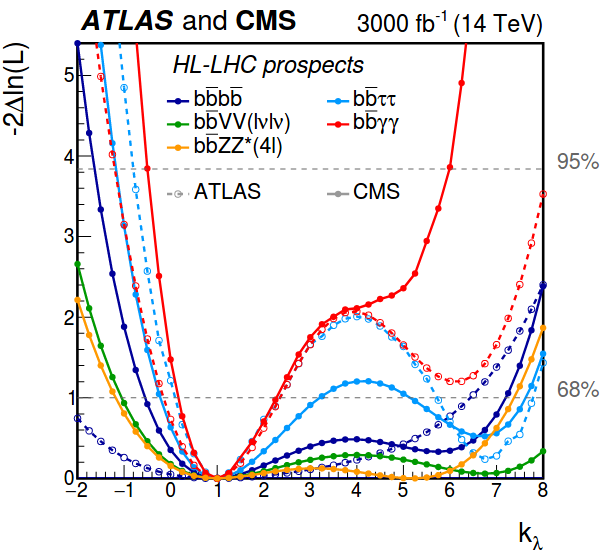
\includegraphics[width=0.46\textwidth]{Figures/HiggsPairProduction/projection2.png}}
\subfloat[]{\centering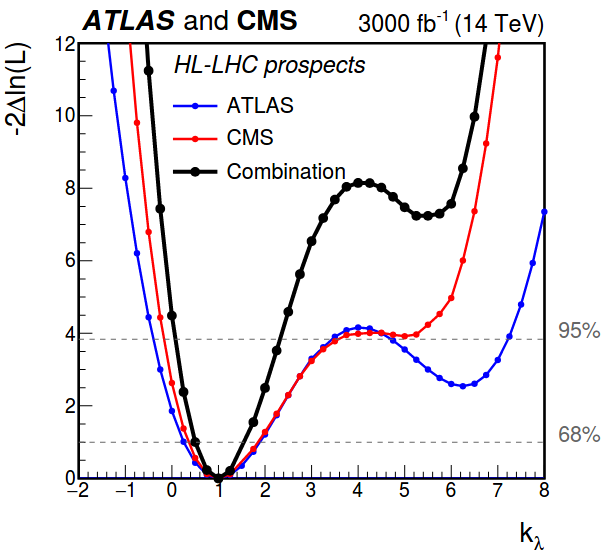
\includegraphics[width=0.46\textwidth]{Figures/HiggsPairProduction/projection1.png}}
\caption[Minimum negative-log-likelihood as a function of the $\kappa_{\lambda}$ modifier obtained by performing a fit to the expected background and SM signal]{Minimum negative-log-likelihood as a function of the $\kappa_{\lambda}$ modifier obtained by performing a fit to the expected background and SM signal~\cite{yellowreport}. A) Contours for different channels in the ATLAS and CMS projections, represented in dashed and solid lines, respectively. B) Combined results (black) from the CMS (red) and ATLAS (blue) projections.}
\label{fig:coklprojection}
\end{figure}
